\documentclass[8pt, twocoloumn]{article}
	\usepackage[left=2.5cm, right=2.5cm, top=2.5cm, bottom=1.5cm]{geometry}

    \title{\textbf{Geometric Phase in Quantum Theory: 
    A Review}}
    
    
    \author{prikarsartam}
    \date{02.08.2021}
    

\usepackage{amsmath}
\usepackage{amsthm}
\usepackage{amsfonts}
\usepackage{amssymb}
\usepackage{hyperref}
\usepackage{chngcntr}
\usepackage{braket}
\usepackage{esint}
\usepackage{graphicx}
\usepackage{lipsum}
\usepackage{docmute}





\begin{document}

\newtheorem*{theorem}{Definition}
\newtheorem*{axiom1}{Axiom 1}
\newtheorem*{axiom4}{Axiom 4}
\newtheorem*{definition1}{Adiabatic Evolution}
\newcommand\sbullet[1][.5]{\mathbin{\vcenter{\hbox{\scalebox{#1}{$\bullet$}}}}}

\counterwithin{equation}{section}

\maketitle

\begin{abstract}
Born's interpretation of a state and corresponding wavefunction in Quantum Theory being probabilistic and $physically$ unique upto any arbitrary phase; ignores all possible regards of single-system phase-factors of which the dynamical-phase is very well nurtured, but there is another phase factor accompanying a kinematic quantum state only dependent on the geometry of the trajectory in projective Hilbert Space, namely a geometric phase; which could be described from traditional methods in quantum theory starting from adiabaticity of the Hamiltonian then generalizing further on. But interestingly such geometric phases have great mathematical correspondence with holonomy of the $U(1)$ Hermitian line bundle over projective Hilbert space. 
\end{abstract} 





\section{Introduction:}

This article presents the general idea behind Geometric Phase accompanying a wavefunction, its origin, and its further mathematical interpretation. An interesting additional phase factor, that latches onto the wavefunction in any cyclic evolution can be interpreted as holonomy of parallel transport on U(1) principal fibre bundles over $\mathcal{PH}$. It starts with the origin of phase from unitarity, general discussion on Phase of a wavefunction, which follows Geometric phase, and its origin from adiabatic assumption and Berry's phase, later its holonomic interpretation is provided. Lastly its shown there could possibly be additional phase terms, dependent solely on the geometry of corresponding spacetime, and the simplest one among them has been presented. 




\section{Unitarity and Schrödinger's Equation: }
Specific Symmetry corresponds specific invariance, which is reflected upon invariance due to any orthogonal-transformation in classical mechanics or a Unitary Transformation as its general case in Quantum Theory, the underlying idea in both cases is the conservation of any coordinate-independent quantity, i.e. a scalar; which say for a vector, is the norm, or its projection over another such which is formulated to be the inner product between a vector and a covector [could be same for norm of it, or different for projection], and equivalently in Dirac's representation, a ket and a bra. Here the Unitary transformation will be of primary interest and how it validates itself in quantum theory. In this section the Unitarity as well as its relation with Schrödinger's Equation will be elaborated for general time-dependent Hamiltonian and general time-evolution operator will be considered for arbitrary Hamiltonian

Since Schrödinger's and Heisenberg's description of quantum theory, from wave-mechanics and matric-representation point of view, posed severe contradictions, these were partly resolved by Dirac-Neumann Aximatization of quantum theory, where explicitly the pillers of this theory were established. \cite{schuller} as:
Among them, 

the 1st Axiom defines a state of a quantum system, and the 4th one talks about $Unitary \ Dynamics$ which is dynamics of a quantum state where no measurement has been made, and correspondingly the $projective \ dynamics$ describes the situation when any measurement takes place of which not much will be discussed in this paper. 

\begin{axiom1}{\label{axiom1: axiom1}}
(Quantum systems and states) To every quantum state there is associated a seperable complex Hilbert Space $(\mathcal{H}, (+), (.) , \langle . | . \rangle )$ where the states $\rho$ of the system are all positive trace-class linear maps $\rho : \mathcal{H} \to \mathcal{H}$ for which $Tr(\rho)=0$
\end{axiom1}

Where the $trace \ class$ refers to linear maps in $\mathcal{H}$ s.t. $A : \mathcal{H} \to \mathcal{H}$ s.t. for any choice of complete set of bases $(\{e_i\}) \underset{spans}{\in} \mathcal{H}$ $$\sum_{n} \braket{e_n| Ae_n} < \infty$$
Now states can be  $pure$ or $mixed$. A state is $pure$ if 

\begin{equation} \exists \psi \in \mathcal{H} \ s.t. \ \forall\alpha \in \mathcal{H}, \ \rho(\alpha) = \frac{\braket{\psi|\alpha}}{\braket{\psi|\psi}}\psi 
\end{equation}

and $Tr A := \sum_{n} \braket{e_n| Ae_n}$ for some map in $\mathcal{H}$

\begin{axiom4}

(Unitary Dynamics) During a time interval ($ t_1, t_2 \in 	\mathbb{R}$) where no measurement has taken place the states $\rho(t_1)$ and $\rho(t_2)$ are related as: 

$$ \rho(t_2) = U(t_2-t_1) \rho(t_1) \ U^{-1}(t_2-t_1)$$

With the Unitary Evolution Operator defined as:

$$ U(t) := exp(-\frac{i}{\hbar} \int _{t_1}^{t_2}\mathbb{H}(t')dt')$$

where $\mathbb{H}$ is the Energy Observable

\end{axiom4}


Where the definition of $Unitary \ Operator$ says: $\hat{U} \hat{U}^{\dag} \equiv \hat{U} \hat{U}^{-1}= \mathbb{I} $

Where such an Exponential map of operators (which can be represented as matrices), are expressed as:  


\begin{equation}
exp(-\frac{i}{\hbar}\int _{t_1}^{t_2} \mathcal{O}(t')dt')= \sum_{n=0}^{\infty}\frac{1}{n!}(-\frac{i}{\hbar}\int _{t_1}^{t_2} \mathcal{O}(t')dt')^{n}
\end{equation}

It is very fascinating that from these two axioms, the $\textbf{Schrödinger's equation}$ can be $\textbf{derived}$, with these two axioms, for general-time dependent scenario from the Axiom 1, and Axiom 4. 

For some simplicity of calculation, (just notationally) consider: 

\begin{align}
& \mathcal{O}_{\mathbb{H}} := exp(-\frac{i}{\hbar}\int _{t_1}^{t_2} \mathbb{H}(t')dt')  \ \ \ \ \ \ \ \ \\ 
& \mathcal{O}_{\mathbb{H}}^{\dag}=\mathcal{O}_{\mathbb{H}}^{-1}=exp(+\frac{i}{\hbar}\int _{t_1}^{t_2} \mathbb{H}(t')dt') 
\end{align}

We wish to consider the time evolution of a fixed $\psi_0 := \ket{\psi(0)} \to \psi_t := \ket{\psi(t)} \in \mathcal{H}$ 
Therefore Axiom 1 gives us: 
\begin{equation}
\rho_t(\alpha)= \frac{\braket{\psi_t|\alpha}}{\braket{\psi_t|\psi_t}}\ket{\psi_t} = \mathcal{O}_{\mathbb{H}} \rho_0(\alpha) \mathcal{O}_{\mathbb{H}}^{\dag}= \mathcal{O}_{\mathbb{H}} \frac{\braket{\psi_0|\alpha}}{\braket{\psi_0|\psi_0}}\ket{\psi_0} \mathcal{O}_{\mathbb{H}}^{\dag}
\end{equation}

for unique $\ket{\psi_t}$ from $\ket{\psi_0}$ it is evident that [since true $\forall \alpha \in \mathbb{C}$]

\begin{equation}
\ket{\psi_t} = \mathcal{O}_{\mathbb{H}}\ket{\psi_0} \ \ \ \ \ \ \ \  \ \  \bra{\psi_t}=\bra{\psi_0}\mathcal{O}_{\mathbb{H}}^{\dag}
\end{equation}

Therefore, now writing explicitly:




\begin{align}
\ket{\psi_t}
&= exp(-\frac{i}{\hbar}\int _{t_1}^{t_2} \mathbb{H}(t')dt')\ket{\psi_0}= \{ \mathbb{I} -\frac{i}{\hbar}\int _{0}^{t} \mathbb{H}(t')dt' + \frac{1}{2!}(\frac{i}{\hbar})^2 \int _{0}^{t}dt' \int_{0}^{t} dt_1 \mathbb{H}(t_1)\mathbb{H}(t')- \nonumber \\
& \frac{1}{3!}(\frac{i}{\hbar})^3\int _{0}^{t}dt' \int_{0}^{t} dt_1 \int_{0}^{t} dt_2 \mathbb{H}(t_2) \mathbb{H}(t_1)\mathbb{H}(t') + . . .  \ \} \ket{\psi_0} \nonumber \\
& \ket{\psi_t} - \ket{\psi_0} = \{-\frac{i}{\hbar}\int _{0}^{t} \mathbb{H}(t')dt' + (\frac{i}{\hbar})^2 \int _{0}^{t}dt' \int_{0}^{t'} dt_1 \mathbb{H}(t_1)\mathbb{H}(t')-   (\frac{i}{\hbar})^3\int _{0}^{t}dt' \int_{0}^{t'} dt_1 \int_{0}^{t_1} dt_2 \mathbb{H}(t_2) \mathbb{H}(t_1)\mathbb{H}(t') \nonumber \\ 
& + . . .  \ \} \ket{\psi_0}
\end{align}


Here the power series expansion of the exponential map is used, and differentiating, with noting that $\ket{\psi_0}$ is fixed, it shows:  {It is to note that the Hamiltonian's in differnt times need no necessarily commute and maintaining the non-commutative sequence is important}:



\begin{align}
\frac{d}{dt}\ket{\psi_t}= -\frac{i}{\hbar}\mathbb{H}(t) 
\{ \mathbb{I} -\frac{i}{\hbar}\int _{0}^{t} \mathbb{H}(t')dt' + \frac{1}{2!}(\frac{i}{\hbar})^2 \int _{0}^{t}dt' \int_{0}^{t} dt_1 \mathbb{H}(t_1)\mathbb{H}(t')- ... \ \} \ket{\psi_0} \nonumber 
\end{align}

\begin{equation}
= -\frac{i}{\hbar}\mathbb{H}(t) \mathcal{O}_{\mathbb{H}}\ket{\psi_0}
\end{equation}

therefore we Identify our good-old Schrödinger's Equation: 

\begin{equation}{\label{schro}}
 \frac{d}{dt}\ket{\psi_t}=-\frac{i}{\hbar}\mathbb{H}(t)\ket{\psi_t}
\end{equation}

Note that the origin of this is the axioms, which considered the Energy Obsersable, namely, the Hamiltonian which were the generators of time evolution. 
Maybe that is why these postulates are for, to come around the so called underivable portions of the the thory, and bound them all together with the axiom-named \textbf{desiderata} of Quantum Theory. 

\subsection{Phase:}


From the discussion above, two remarks are necessary:

\begin{itemize}
  \item considering $\alpha \in \mathbb{C}$ there are infinite equivalence class $(\{ \alpha\}) \equiv \rho$  representing same pure state for any system.
  \item Now fixing $\alpha$ one sees for $\psi \to \psi' = exp(i \Lambda)\psi$ $$\rho(\alpha) = \frac{\braket{\psi'|\alpha}}{\braket{\psi'|\psi'}}\psi' =  \frac{ exp(-i\Lambda)\braket{\psi|\alpha}}{\braket{\psi|\psi}}exp(i\Lambda)\psi = \frac{\braket{\psi|\alpha}}{\braket{\psi|\psi}}\psi $$ since $\braket{.|.}: \mathcal{H} \times \mathcal{H} \to \mathbb{C}$ where $\Lambda: C^{\infty}(\mathbb{R}) \to \mathbb{R} $ any real function. which also indicate the equivalence class of $(\{ \Lambda \})$ representing same state for the simplest pure quantum system. which will be referred to as Gauge Transformations further with detailed exposure.
\end{itemize}

therefore there are ambiguities from the definition/axiomatization of the states of quantum system upto maintaining Unitarity, the inner-product $\braket{.|.}$ being invariant under such transformation. Also the Schrodinger's equation being a wave-equation, and solution constituting a $probability \ wave$ it must contain a factor, which determines its probabilistic existance of a quantum particle. Something interesting in theories of waves, like Electromagnetism,  Quantum Theory, these being wave-mechanics in one way or the other, are Linear Theories, which directly mean, given a set of solution of that theory's dynamical equation, any linear combination of them would also be a solution of so, \footnote{Newtonian mechanics even General relativity being highly non-linear they don't support superposition principal} gives one the $\textbf{
Superposition Principal}$ which is the basis of how phases interfere, and manifests their wave-nature. 

Consider a simple situation, two normalized wave-kets differing by some phase factor is superposed. 

\begin{align}
    \ket{\Psi} &= (\ket{\psi} \ e^{i \alpha} + \ket{\psi} \ e^{i \beta})  \\
    &= \ket{\psi}(e^{i \alpha} + e^{i \beta}) = \ket{\psi}(e^{i (\alpha - \beta)} + 1) e^{i\beta} 
\end{align}

Now from Born's interpretation being mod-square of a wavefunction as its probabilistic measure, one can write:

\begin{align}{\label{interference}}
    |\braket{\Psi|\Psi}|^{2} = |\braket{\psi|\psi}|^{2}(1+cos(\alpha - \beta)) 
\end{align}

Now $\psi$ being a normalized state: $|\braket{\psi|\psi}|^{2} = 1$ Therefore one readily sees: the probabilistic picture of the superposed state changes $co-sinusoidally$ which is the reason behind specific pattern in wave-interference.  But phase of a wavefunction is never an observable entity, but what is so, is the Relative Phase. Which can be accumulated by so many possible reasons. 

It can be very simply argued how, every manifestation of the environment over a quantum system causes the change in phase of its wavefunction. The reason is as follows:

The wavefunction is always a normalized quantity, since it represents its own probabilistic existance in either position space (mostly relatable) or momentum space (not so much). Therefore when certain change it its physical environment takes there's no meaning in the change of its norm, since, that's unity, rather it's the phase that gives the distribution of probability of that wavefunction. But still why then the norm keeps invariant? well, that's only for a pure state, since there's none else to compare its phase, which can only happen when two different-phased wavefunction would superpose and then indeed the relative phase, like \ref{interference} would reflect its physicality. It's just now $pointwise \ determinism$ like newtonian one, it's indeed deterministic, but it's $probabilistic \ determinism$ where one can think the $determinism$ being spread out of point, and giving distribution around it. 

Consider this, the electromagnetic Hamiltonian is given as $\hat{H} = {(\frac{\hbar}{i}\nabla - \frac{q}{c}A)}^{2}$ and then the Schrodinger equation takes the form as \ref{electromagneticschrodingereequatinon}. 

And one can directly see, for change in gauge for electromagnetic potentials, as: $A^{\mu} \to A'^{\mu} = A^{\mu} + \frac{\partial}{\partial x^{\mu}}\Lambda(x^{\mu})$ the wavefunction changes as: 

\begin{align}
    \psi(x^{\mu}) \to \psi'(x^{\mu})= \psi(x^{\mu}) \ e^{\frac{iq}{\hbar c} \Lambda(x^{\mu})}
\end{align}

One can directly prove that as either putting it in the Schrodinger equation and check if true OR, can consider (since gauge transformation doesn't change classical picture) an Unitary transformation between normal wavefunction and the gauged one, and then solve it with schrodinger equation for Hamilton with gauge transformed potential, then one can straightforwardly find the Unitary Operator being a phase as $e^{\frac{iq}{\hbar c} \Lambda(x^{\mu})}$.

In case of $\textbf{Aharanov-Bohm Effect}$ with field free region, one can consider (since $\nabla \times A = B = 0$) $A = \nabla \Lambda$ i.e. the potential is purely a gauge. Then $\Lambda = \int^{x_f}_{x_i} \vec{A}.d\vec{r} = \int^{f}_{i} A_{\mu}dx^{\mu}$

Now for an interference phenomenon where the two wavefunction trajectories enclose a definite surface, perpendicularly through which runs a non-zero magnetic flux, the classical motion although being unaltered, the superposition gives:

\begin{align}
    \Psi &= \psi \ exp \left[ \int^{f}_{i, \ path \alpha} A_{\mu}dx^{\mu} \right]+  \psi \ exp \left[\int^{f}_{i, \ path \beta} A_{\mu}dx^{\mu} \right]\\
    &= \psi\  \Bigg\{ exp \left[ \oint  A_{\mu}dx^{\mu}\right]  + 1\Bigg\} e^{(\int^{f}_{i, \ path \beta} A_{\mu}dx^{\mu})}
\end{align}

Where the additional relative phase: $\oint  A_{\mu}dx^{\mu}$ is the $\textbf{Aharonov-Bohm Phase}$
\section{Geometric Phase:}

As mentioned previously, the inner product, mostly destroys the information of the $accumulated \ phase$ during any process. Also the $\textbf{dynamical Phase factor}$ solely depends on the Hamiltonian and it's corresponding eigenspectrum for any evolution that is maintaining the Schrodinger's equation of corresponding Hamiltonian. It is important to note the instantaneous eigenstates of the Hamiltonian operator, in general, need not be the solution of the Schrodinger's equation with same $\mathbb{\hat{H}}$, which reflects only time-independent scenario. But more is there than met by the inner product $\braket{.|.}$, and one among them, is only governed by the geometry of kinematic trajectory of the system.
(for our consideration, only pure states will be of interest)
[Throughout here $\psi_n$ would refer Instantaneous Eigenstate and $\Psi$ to the solution of Schrodinger equation]

Consider a Hamiltonian depending on several parameters: $h(\textbf{R}_t)$ and its instantaneous Eigenspectrum :

\begin{align}{\label{eigenstate}}
\begin{split}
    h(\textbf{R}_t) \ket{\psi_n (\textbf{R}_t)} ={}& E_n(\textbf{R}_t) \ket{\psi_n (\textbf{R}_t)} \notag
\end{split}\\
\begin{split}
    \braket{\psi_n (\textbf{R}_t)| \psi_m (\textbf{R}_t)} ={}& \delta_{nm}
\end{split}
\end{align}

And the finite-dimensional spectral resolution reads, defining the projection operator: 

\begin{align}
\begin{split}
\Lambda_n(\textbf{R}_t):= \ket{\psi_n(\textbf{R}_t)}\bra{\psi_n(\textbf{R}_t)} 
\end{split}\\
\begin{split}
h(\textbf{R}_t)={}& \sum_{n}^{dim\mathcal{H}} E_n(\textbf{R}_t)\Lambda_n(\textbf{R}_t) 
\end{split}
\end{align}
Thus for dependencies of the parameters, any observable of the system are as well linear operators with $\textbf{R}_t$ as argument and assuming them being single valued, that repetition of $\textbf{R}_t$ would yield repition of eigenvalues of that operator, therefore single valuedness of the operators are another way of waying strich dependence of the parameters, and none else.
Since this article concerns only about cyclic evolution, thus it requires to be clearly mentioned. 

A $\textbf{Cyclic Evolution}$ is one where the initial quantum state evolves periodically in time, therefore the periodicity of dependencies (parameters) of any state. would give periodicity of the state (for single-valued ones). If the environmental process is periodic thus traverses a closed loop $\textbf{C} \in M$ where $M$ is to be considered the $\textbf{parameter space}$
\begin{align}
\textbf{C}_t: t \in [0,T] \subset \mathbb{R} \to M \ \ \ \textbf{C}_0=\textbf{C}_1
\end{align}
Therefore single-valuedness of the observables indicate 

\begin{align}
\begin{split}
h(\textbf{R}_0)= {}& h(\textbf{R}_T) \notag 
\end{split}\\ 
\begin{split}
 E_n(\textbf{R}_0)= {}& E_n(\textbf{R}_T) \notag 
\end{split} \\
\begin{split}
\Lambda_n(\textbf{R}_0) ={}& \ket{\psi_n(\textbf{R}_0)}\bra{\psi_n(\textbf{R}_0)}  = \ket{\psi_n(\textbf{R}_T)}\bra{\psi_n(\textbf{R}_T)}  = \Lambda_n(\textbf{R}_T) 
\end{split}
\end{align}

It is notable here that there could possibly be nothing that gurantees the eigenbases $\ket{\psi(\textbf{R}_t)}$ to be single valued, but only unique upto a phase factor and with substituting:

\begin{align}
\ket{\psi_n(\textbf{R}_T)}=exp(i\Lambda_n)\ket{\psi_n(\textbf{R}_0)} \ \ \ \ \Lambda_n \in \mathbb{R}
\end{align}
It definitely shows, even with this substitution, the physical observability of the processes with singl-valued observables are invariant with such a $\textbf{phase transformation}$ for cyclic systems, where it it evident how an additional phase factor during cyclic evolution indeed turns out to be plausible from the formalism and necessary conditions for physicality. 

Threrefore it is possible for arbitrary such phase transformation 

\begin{align} {\label{gau}}
\ket{\psi_n(\textbf{R}_t)} \to \ket{\psi_n(\textbf{R}_t)}'=e^{i\Lambda_n}\ket{\psi_n(\textbf{R}_t)}
\end{align}

and see that the transformed states serve equally as the instantaneous eigenstates of the system's Hamiltonian. 
In the further subsections, such periodicity of states with respect to the parameters it depend on, from the Hamiltonian will be elaborated under certain conditions of our concern.
\subsection{Adiabaticity: }
The idea behind Adiabaticity in quantum theory, that it turns out to be celebrated corollary of Schrödinger's Equation, origianally identified by M.Born and V.A.Fock in 1928, that for a general Hamiltonian with parameters keeps the initial eigenstates (very closely) invariant under time-evolution.  

Considering simplest classical correspondence: that a simple harmonic pendulum, which is swinging in some frequency, will almost maintain it (and all its physical characteristics) if the whole system is VERY SLOWLY moved from one place to another. For our general-time and parameter dependent Hamiltonian (time dependency of the Hamiltonian is induced implicitly through parameter i.e. $ \mathbb{H}_t \equiv \mathbb{H}(\textbf{R}_t)$)
There are extensive sophisticated mathematical backgroud to this general-adiabatic scenario and corresponding theorems, which will not be of much concern here, rather its idea will be somewhat simply provided within this framework. 
\begin{definition1}
For a very slowly varying Hamiltonian, the system remains to be the initial eigenstate of the Hamiltonian at any time during its evolution.
\end{definition1}
It is evident from \ref{eigenstate} and from Schrödinger evolution of the state: 

\begin{align}
\ket{\Psi_0}\bra{\Psi_0} = \ket{\psi_n(\textbf{R}_0)}\bra{\psi_n(\textbf{R}_0)} = \Lambda_n(\textbf{R}_0))
\end{align}
Projection operators of these pure states are more important since the states themselves are unique upto some phase factors [which indeed will be the concerns here], and noting Schrödinger's equation's solution can only be the corresponding Hamiltonian's eigenstate if the system is a stationary one, which for general case that this article is interested toward is not, therefore for $t=0$ one can consider such.

The proof of this Adiabatic theorem will not be discussed herewithin, an interested reader can find it in \cite{adiabaticberry}. Considering the result of the Adiabatic Theorem it it then evident that
\begin{align}{\label{we}}
W(t) := \ket{\Psi_t}\bra{\Psi_t} \overset{adiabatic}{=} \ket{\psi_n(\textbf{R}_t)}\bra{\psi_n(\textbf{R}_t)}=\Lambda_n(\textbf{R}_t)
\end{align}
Again consideration of pure-state projection operator is to point that the states themselves can be arbitrarily phase-differef, though their projection operators are intact, which can be well interpreter in terms of $Projective \ Hilbert \ Space$
If considered $W_{\psi} := \ket{\psi}\bra{\psi}$ to be pure-state projection operators $\forall \psi \in \mathcal{H}$
then the Projective Hilbert Space is defined to be: 

\begin{align}
\mathcal{PH}:= \set{\ket{\psi}\bra{\psi}|\forall \psi \in \mathcal{H}}
\end{align}
Therefore it's clear from here that: $\psi \to \psi_1 = \psi \ exp(i\alpha) \implies W_{\psi} = W_{\psi_1}$, and since the phase factors $exp(i\alpha) \ \forall \alpha \in \mathbb{R}$ are the member's of the 1-paramter family of Unitary Transformations $U(1)$ or simply the lie group $U(1)$ it's formal to consider: $\mathcal{PH}= \mathcal{H}/ U(1)$ more of which will be discussed in later chapters.

therefore the adiabatic assumption gives us that is $\textbf{R}_t$ traverses some cyclic or closed path in the Parameter Space then the pure-states corresponds to a closed curve $\Lambda_n(\textbf{R}_t)$ \ref{we} in $\mathcal{PH}$
Therefore the cyclic traversal eigenprojectors in $\mathcal{PH}$ represent cyclic travrsal of eignstates  
$\ket{\psi_n(\textbf{R}_t)}$ BUT, upto some phase; which turns out to play very significant  role and has several interesting properties. 

At this point, expressing the state vectors $\ket{\Psi_t}$ in terms of the hamilton's instantaneous eigenbases $\{\psi_n(\textbf{R}_t)\}$, considering adiabatic assumption to hold for the hamilton to vary very slowly, one can write:

\begin{align}
\ket{\Psi_t}=c_n(t)\ket{\psi_n(\textbf{R}_t)}
\end{align}
for some constant $c_n(t) \ \forall t,n$, since \ref{we} says such a constant is required, provided $c^*_n(t)c_n(t)=\mathbb{I}$ there one hindsight definitly says $c(t) \in U(1)$ which will be investigated here: [noting that $c(0)=\mathbb{I}$] Substituting the relation in Schrödinger's equation and using \ref{eigenstate} yields:

\begin{align}
i\hbar \sum_{n}(\dot{c}_n\ket{\psi_n(\textbf{R}_t)}+c_n \ket{\dot{\psi_n}(\textbf{R}_t)})=\sum_{n}E_n(t)\ket{\psi_n(\textbf{R}_t)}
\end{align}

Therefore inner-product of this expression with $\bra{\psi_m(\textbf{R}_t)} \ for \ some \ m \neq n$ also keeping in mind that eigenvectors of a Hermitian Operators are orthogonal i.e. $\braket{\psi_m(\textbf{R}_t)|\psi_n(\textbf{R}_t)}=0 \ \forall m\neq n$ 

\begin{align}{\label{ffs}}
i\hbar \dot{c}_m=(E_m(t)-i\hbar \braket{\psi_m(\textbf{R}_t)|\dot{\psi}_m(\textbf{R}_t)})-i\hbar\sum_{n}\braket{\psi_m(\textbf{R}_t)|\dot{\psi}_n(\textbf{R}_t)}
\end{align}

Now $\braket{\psi_m|\dot{\psi}_n}$ is related to the matrix element of the Hamiltonian $H(\textbf{R}_t)$ in its Eigenspace as \cite{berrypaper}, taking derivative of the \ref{eigenstate} we obtain:

\begin{align}
\dot{H}(\textbf{R}_t)\ket{\psi(\textbf{R}_t))}+H(\textbf{R}_t)\dot{\psi}(\textbf{R}_t))=\dot{E_n}(\textbf{R}_t)\ket{\psi(\textbf{R}_t)}+E_n(\textbf{R}_t)\dot{\psi}(\textbf{R}_t))
\end{align}

again taking inner product with $\bra{\psi_m(\textbf{R}_t)} \ m\neq n$ gives:

\begin{align}
\braket{\psi_m|\dot{H}|\psi_n}+\braket{\psi_m|H|\dot{\psi}_n}= \braket{\psi_m|\dot{H}|\psi_n}+E_m\braket{\psi_m|\dot{\psi}_n}=E_n\braket{\psi_m|\dot{\psi}_n}
\end{align}

thus obtaining:
\begin{align}
\braket{\psi_m(\textbf{R}_t)|\dot{\psi}_n(\textbf{R}_t)}= & \braket{\psi_m|\dot{H}(\textbf{R}_t)|\psi_n} \over E_n(t) - E_m(t)
\end{align}

plugging it back to \ref{ffs}:

\begin{align}
i\hbar \dot{c}_m=(E_m(t)-i\hbar \braket{\psi_m(\textbf{R}_t)|\dot{\psi}_m(\textbf{R}_t)})-i\hbar\sum_{n} & \braket{\psi_m|\dot{H}(\textbf{R}_t)|\psi_n} \over E_n(t) - E_m(t)
\end{align}

Here the most crucial consideration of Adiabaticity comes about, namely, for VERY slowly varying Hamiltonian it is evident that $\frac{d}{dt}H \to 0$
Thus neglecting the 2nd term it's found:

\begin{align}
\begin{split}
c_m(t)={}& c_m(0) \ exp \ \Big\{ \frac{1}{i\hbar} \int^{t}_{0}(E_m(t')-i\hbar \braket{\psi_m(\textbf{R}_t)|\dot{\psi}_m(\textbf{R}_t)})dt' \Big\} \notag 
\end{split} \\
\begin{split}
={}& c_m(0) \ exp \ \Big\{ -\frac{i}{\hbar} \int^{t}_{0}E_m(t')dt' \Big\} \ exp \ \Big\{i\int^{t}_{0}i\braket{\psi_m(\textbf{R}_t)|\dot{\psi}_m(\textbf{R}_t)}dt' \Big\}
\end{split}
\end{align}

Just renaming:

\begin{align}
\eta(t)=-\frac{1}{\hbar} \int^{t}_{0}E_m(t')dt'  \ \ \ \ \ \ \ \  \gamma_m(t)=\int^{t}_{0}i\braket{\psi_m(\textbf{R}_t)|\dot{\psi}_m(\textbf{R}_t)}dt'
\end{align}

therefore our state now looks: 

\begin{align}{\label{state}}
\ket{\Psi_t}=c_n(0) \ e^{i\eta_n(t)}\ e ^{i\gamma_n(t)} \ket{\psi_n(\textbf{R}_t)}
\end{align}

Now it doesn't stop here, rather the whole story starts from this point. 
In this section the adiabatic approximation of a quantum state has been considered, it's further implications will now jump to the section.

\subsection{Berry's Phase: }

It has been presented how adiabaticity and cyclicity of quantum state gives rise to additional phase difference between the initial and final state. Since they are phase factors, they belong to th 1-parameter family of Unitary transformations or U(1) lie group, thus considering pure state eigenprojctors, one achieves back the initial states. 
The phases obtained so far are $\eta$ and $\gamma$ where the latter is of crucial interest, and will considered upto a length, and the first one is well-known Dynamical Phase Factor, which is just accompanying signature of time-evolution. 

The other phase factor, namely $\gamma_n := \textbf{geometric phase}$ craves greater attention, and since it was first mentioned by M.V.Berry in 1984 \cite{berrypaper} it is also well known to be Berry's Phase.

The derived additional phase 

\begin{align}
\gamma_n(t)=\int^{t}_{0}i\braket{\psi_n|\dot{\psi}}dt'
\end{align}
with $\ket{\psi_n}$ to be the instantanous eigenstates of the Hamiltonian is a completely real number, i.e. 

\begin{align}
Im \ \braket{\psi_n|\dot{\psi}} \in \mathbb{R}
\end{align}

Since considering $\braket{\psi_n|\psi_n}$ to be a constant it is easy to show 

\begin{align}
\braket{\psi_n|\dot{\psi}}^* = -\braket{\psi_n|\dot{\psi}}
\end{align}

which clearly indicates$ \braket{\psi_n|\dot{\psi}}$ is $\textbf{purely imaginary}$.

Another very significant properties of the phase angle $\gamma_n(t)$ is that it doesn't depend on time at all, rather the time-integral can be expressed as a curve-intgral over a vector valued quantity:

\begin{align}{\label{berryconnection}}
\begin{split}
\gamma_n(t) ={}&\int_{0}^{t} i \braket{\psi_n(\textbf{R}_t')|\frac{d}{dt'}|\psi_n(\textbf{R}_t')}dt' = \int_{0}^{t} i \braket{\psi_n(\textbf{R}_t')|\frac{\partial}{\partial \textbf{R}^{\mu}}|\psi_n(\textbf{R}_t')}\frac{\partial \textbf{R}^{\mu}}{\partial t'}dt' \notag
\end{split}\\
\begin{split}
={}& \int_{R_0}^{R_t} A^n_{\mu}(\textbf{R}_t)d \textbf{R}^{\mu} \ \ \ \ \ \ \ \ \ \ \ A^n_{\mu}(\textbf{R}_t) = i \braket{\psi_n(\textbf{R}_t')|\nabla|\psi_n(\textbf{R}_t')}
\end{split}
\end{align}

Therefore the term is independent of the dynamical features of the system (time-energy) rather completely kinematic one, noting that $\nabla$ here is a Gradient operator in the parameter space.
This vector valued quantity is extremely analogous to electromagnetic vector potential and even will be exactly in such cases, these functions $A^n$ can be defined only with single-valued eigenbases, and since it is tough to find such set of eigenbasis throuout the process or everywhere on the parameter space, it is to be assumed and thus defined over a patch in parameter space where th curve $C$ lies and a set of smooth and single-valued eigenbasis of the Hamiltonian exists.
This Vector valued function can be written as a local-connection-one form [local, since its locally defined in the parameter space, connection, since it induces a rule for paraller transport along this curve in parameter space to the fibre bundles of the Hilbert space, which will be elaborated shortly in following sections]

\begin{align}{\label{oneform}}
A^n= A^n_\mu \ dR^{\mu}=\braket{\psi_n(R_t')|\frac{\partial}{\partial R^{\mu}}|\psi_n(R_t')}  dR^{\mu}=\braket{\psi_n(R_t)|\textbf{d}|\psi_n(R_t)}
\end{align}

where $d$ is the exterior derivative which is defined on the same patch where $\ket{\psi_n}$ are defined within, this one form is regarded as the $ \textbf{Berry's connection one form}$ with which the expression for the phase angle simplifis to: 

\begin{align}
\gamma_n(t)=\int_{R_0}^{R_T}\braket{\psi_n(R_t)|\textbf{d}|\psi_n(R_t)} = \int_{\textbf{C}}A^n \ \ \ \ \ \ \to \oint_{\textbf{C}}A^n
\end{align}
The loop integral for the situation where the parameters run a loop i.e. $R_T = R_0$ and since the $A^n$ one form is not an exact one form [it's notrepresentable to be exterior derivative of something] its contour integral might not vanish within a loop, and therefore it is physically existant a phase angle of a quantum state, and how it observably manifest will be discussed in Aharonov-Bohm context. 

From the viewpoint of \ref{gau} the additional phase factors might possibly be Gauged away, by such phase transformations but it has several restrictions of which is part is all about.

From the definition of such vector valued function of our concern \ref{berryconnection} and for gauge-transformations of such kind \ref{gau} it craves attention to see what happens: 

\begin{align} {\label{gaugeinvariance11}}
\begin{split}
A^n_{\mu}(R_t) \to A'^n_{\mu}(R_t) ={}& i \braket{\psi_n (R_t)|'\nabla|\psi_n(R_t)}'
\end{split} \notag \\
\begin{split}
={}& i \braket{\psi_n(R)e^{-i\Lambda_n(R)}|\nabla | \psi_n(R)e^{i\Lambda_n(R)}}
\end{split} \notag  \\
\begin{split}
={}& i \braket{\psi_n (R_t)|\nabla|\psi_n(R_t)} + i e^{-i\Lambda_n(R)}(\nabla e^{i\Lambda_n(R)})
\end{split} \notag \\
\begin{split}
\textbf{A}'^n_{\mu}(R_t) = \textbf{A}^n_{\mu}(R_t)-\nabla \Lambda_n(R)
\end{split}
\end{align}

Likewise the connection one-form transforms as \ref{oneform}:

\begin{align}
A^n \to A'^n = A^n - d\Lambda_n(R)
\end{align}
 
Therefore the phase angle transformes as: 

\begin{align}{\label{gaugecheck}}
\begin{split}
\gamma_n(C) \to \gamma'_n(C)={}& \int_{R_T}^{R_0}A'^n(R)dR 
\end{split} \notag \\
\begin{split}
={}&\gamma_n(C)-\Lambda_n(R_T)+\Lambda_n(R_0) 
\end{split}
\end{align}

At this point for most general cases for such a phase accumulation, it is possible to choose a phase transformation to remove that additional phase and get back the expressions as of \ref{state} and \ref{gau} only with the dynamical phase factor, and no such geometric one. 
But very important aspect of this is that for a closed loop with $R_T=R_0$ one readily sees the Geometric phase is $\textbf{gauge invariant}$ i.e. from \ref{gaugecheck}

\begin{align}
\begin{split}
\gamma_n(R)=\gamma'_n(R)
\end{split}
\end{align}

since the additional gauge factors $\Lambda_n(R)$ are single valued, and cannot be removed anyway, it is also evident that gauge independent terms are physically well-observable and indeed that is the case here.

Like classical electromagneticsm $A^n(R)$ is gauge-sensitive but there are terms involved, i.e. Geometric phase for a cyclic evolution, which are not susciptible gauge factors at all. This phenomenon is well explain through Gauge Theory with structure group U(1) and Local Gauge Connection-one-form as $A^n(R)$

In analogy with classical vector potential, th gauge field strength can be given as:

\begin{align}{\label{dafg}}
\begin{split}
F^n := \frac{1}{2}F^n_{ij}dR^i \wedge dr^j = \frac{\partial A^n_j}{\partial R^i}dR^i \wedge dr^j=dA^n
\end{split}
\end{align}

Again the idea of wedge product from diff geometry has been considered here defining the fields strength tensor, and componentwise it is:

\begin{align}
\begin{split}
F^n_{ij} = \frac{\partial }{\partial R^i} A^n_j - \frac{\partial }{\partial R^j} A^n_i \ \ \ \ \ \ \ \ \ \ i,j= 1, 2,.. dim M
\end{split}
\end{align}
here the antisymmetry of wedge product has been considered and this field strength is named as $\textbf{Berry's }$ $\textbf{curvature}$ $\textbf{2-form}$ thus in terms of the eigenbasis it is given as:

\begin{align}
\begin{split}
F^n = d(i \braket{\psi_n|d|\psi_n})= i(d\bra{\psi_n}) \wedge d\ket{\psi_n}
\end{split}
\end{align}
Where one identity of exterior derivative has been used that $d^2=0$

One siginificant property of the curvature 2-form is that, unlike the connection 1-form, it is well and fine gauge-invariant which one can see directly from:


\begin{align}
\begin{split}
F^n \to F'^n = dA'^n=dA^n - d^2 \Lambda_n = dA^n = F^n
\end{split}
\end{align}
Therefore the geometric phase can also be expressed in terms of the local curvature 2-form from the stokes theorem that the line integral, in terms of surface integral

\begin{align}
\begin{split}
\gamma_n(C)=\oint_{C=\partial S}A^n=\int_{S}dA^n = \int_{S}F^n
\end{split}
\end{align}
The surface here $S$ cab be chosen arbitrarly as long as it is encompassed by the curve, that our state traverses. 

It becomes clear when one example is presented and corresponding analogy will make more sense in the following section. Consider a system that depends on 3 parameters \footnote{for simplest one: consider H=-$\vec{\mu}.\vec{B}$ a particle with spin, in magnetic field, the Hamiltonian only depends on the $\vec{B}=(B_1, B_2, B_3)$, 3 external variables determining the dynamics, where spin configuration is the internal one.} the corresponing parameter space is 3-dimensional $M \subset \mathbb{R}^3$ then the dual 3-vector to $F^n$ can be defined as such:

\begin{align}
\begin{split}
F^n_i :={}& \frac{1}{2} \epsilon_{ijk}F^n_{jk}
\end{split}
\end{align} 

with $\epsilon_{ijk}$ being the totally antisymmetri levi-civita symbol and And in vector notation this is simply $F^n = \nabla \times A^n$ which from electromagnetic analogy one find clear similarity between vector potential and magnetic field and the magnetic field indeed defined in terms of the electromagnetic dual-energy-momentum tensor. Which again indicates how $F^n$ must be a gauge invariant qunatity since curl of gradient just goes away, that's somewhat different way of saying the most general $d^2=0$. This will manifest clearly in the following section.

The Geometric phase thus obtained here solely depends on the trajectory in the parameter space and no other things, except the eigenstates themselves which can be chosen to be smooth and single-valued over some patch of the parameter space where the trajectory lies, upon this consideration, it is evident, that single-valuedness of the operator imposes a phase-factor to the initial statevector of a quantum system, though the probability-distribution of such single state is unchanged since the change here is an element of U(1), nevertheless it might be of significant manifest is there are interference between differently-phase-transformed states, and then clearly the extra terms would be well visible physically, and one can get the hunch already that the geometric phase is gauge invariant.
 

\subsection{Aharonov-Bohm Effect: }

\begin{figure}[h!]
\begin{center}
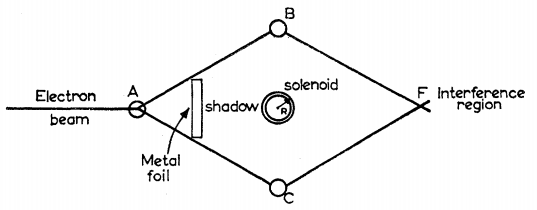
\includegraphics[scale = 0.4]{vectorAB.png}
\hspace{0.2in}
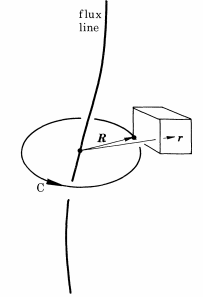
\includegraphics[scale = 0.5]{berryAB.png}
\caption{Phase transformation due to magnetic flux in inaccessible region due to either traversal for two quantun states from either of the sides, or by looping around the flux line, even when $\vec{B}=0$}
\end{center}
\end{figure}


There entails several geometric and topological aspsects of quantum dynamics, and so the geometric phase is no else of that.
Aharonov-Bohm in 1959 pointed out the significane of Electromagnetic potential in quantum theory, where it might act on the system, one bizzare aspect of of electromagnetic potential's manifestation were noted and explained. 
The phenomenon is as follow: consider an interference phenomenon, where two beams come from two slits, and interfere at some screen. The interference patter is due to the relative phase of the wavefunction at different point over scree. Therefore it it evident that the change in relative phase between the two wavefunctions would induce additional effect from the usual interference phenomenon which is namely an interference-fringe-shift.

Now consider a vertical infinitely long current carrying solenoid just behind the two slits as figure 1 from above. It is true that an ideal solenoid has all its magnetic field lines along its axis within its boundary such that no magnetic field lines leak out from the interior of it. And since the magnetic field is perpendicular to the trajectory of the electron beams or the wavefunction of our concern, classically there's no dynamical effect due to Lorentz Force law, but there are more than met by the classical mechanics. Namely the interference fringes shift by a amount proportional to the magnetic flux through the surface contained by the two trajectories. Since the dynamics of the system is unchanged, by only changing the interference term must be some phase-transformation, due to addition of the electromagnetic potential to the Hamiltonian. Likewise it will be shown that this $Aharanov \ Bohm \ Phase$ is equivalent to the $Dirac Phase$ or the electromagnetic $phase$ induced by the electromagnetic Hamiltonian.

From the Gauge transformation of the wavefunction, it has been mentioned how addition to the electromagnetic potential to the Hamiltonian of a system induces an additional phase of the wavefunction, and how that manifest along a closed loop according to a contour integral. Here a more general description of that effect will be presented. 

Consider the Weyl-Heisenberg Algebra or the Canonical-Commutation relation [CCR]: 

\begin{align}
\begin{split}
[X^i , X^j]={}& 0 \notag
\end{split} \\
\begin{split}
[P^i , P^j]={}& 0 \notag
\end{split}\\
\begin{split}
[X^i , P^j]={}& i\delta^{ij} \mathbb{I} 
\end{split}
\end{align}

It is well known the irreducible representation of the Weyl-Heisenberg algebra is Unitarily equivalent to Schrodinger' representation of the operators namely $\braket{x|X^i|\psi}=x^i\psi(x)$ and $\braket{x|P^i|\psi}=-i\hbar\frac{\partial}{\partial x^i}\psi$
But that is not all since there are infinite number of unitary adjoint tranformation of the representation, of type, namely it is evident how unitary transformation of such kind, $\psi \to \psi'=U\psi$ diagonalizes the corresponding Hermitian Operator as $A \to A'=U^{\dag}AU$ for $\psi$ being the eigenbasis of the operator.

Correpondingly considering a unitary operator $U \overset{def}{=} exp(if(\hat{x}))$ the unitary transformation of the Schrodinger representation gives: 

\begin{align}
\begin{split}
\braket{x| X^i|\psi} \to \braket{x|X'^i|\psi} = \braket{x|U^{\dag}X^i U|\psi} = \braket{x| X^i|\psi} = x^i \psi(x)\notag
\end{split} \\
\begin{split}
\braket{x| P^i|\psi} \to \braket{x|P'^i|\psi} = \braket{x|exp(-if(\hat{x})) \ (-i\hbar \frac{\partial}{\partial x^i}) \ exp(if(\hat{x}))|\psi} = \braket{x| X^i|\psi} \notag
\end{split} \\
\begin{split}
={}& (-i\hbar \frac{\partial}{\partial x^i} + \hbar \frac{\partial f}{\partial x^i})\psi(x)
\end{split}
\end{align}

This additional term in the position of representation of the CCRs are due to the unitary equivalance of Schrodinger's Equation which was due to Stone-Neumann's uniquness theorem, that the irreducible representation of the Weyl-Heisenberg Algebra is unique unto unitary equivalance.

Now one can consider the additional term to be in general the coefficients of a one form namely 

\begin{align}{\label{huhuhuhu}}
\omega = \omega_i dx^i, \ \ \ \ \ \ \ \ \ \ \omega_i:=  \hbar \frac{\partial f}{\partial x_i}
\end{align}

just in other words it says: $\omega = df$. This and the CCRs say evidently:

\begin{align}
\partial_i \omega_j - \partial_j \omega_i = 0
\end{align}
Therefore noting that its extrior derivative vanishes out: 

\begin{align}
d\omega = \partial_i \omega_j dx^i \wedge dx^j
= \frac{1}{2}(\partial_i \omega_j - \partial_j \omega_i ) \ dx^i \wedge dx^j
\end{align} 
considering the anti-symmetry property of the wedge product here, which says they are $closed$ one forms, even though theu cannot be always represented as an exterior derivative of another quantity for arbitrarily dimensional parameter space. 

It follows from $Poincare \ Lemma$ that: Every closed p-form in an open ball in $\mathbb{R}^n$ is an exact p-form $\forall 1 \leq p \leq n$. But that's too much to ask for arbitrary system, that the parameter space cannot be such $\mathbb{R}^n$ rather some-define manifold where the one form $\omega$ will manifest finely, and in general cannot be removed away.

One way to see the same thing is to consider the Lagnrangian for a free particle and for a particle in electromagnetic vector-potential, therefore the latter one has additional $\frac{q}{c}A_i \dot{x}^i$ therefore the Canonical momentum for $\mathcal{L}_{free}$ and $\mathcal{L}_{em}$ are respectively:

\begin{align}
\begin{split}
p_{i \ can}^{free} := \frac{\partial \mathcal{L}_{free}}{\partial \dot{x}^{i}}  =m\dot{x}_{i} \ \ \ \ \ \ p_{i \ can}^{em} := \frac{\partial \mathcal{L}_{em}}{\partial \dot{x}^{i}} = m\dot{x}_{i}+\frac{q}{c}A_i \notag
\end{split} \\
\end{align}

the mechanical momenta, in terms of canonical momenta takes form as: 


\begin{align}{\label{hiii}}
\dot{x}^{em}_{i} = \frac{p_i}{m} - \frac{q}{cm}A_i 
\end{align}

with natural units we find exact correspondence between the coefficients of one-form (from 1.39) induced in the momentum-operator-representation is  $\frac{q}{c}A_i $ which indeed is non removable in general unless no potential at all.



Physically intereting the momentum operator says they they are generators of translation of quantum state in the configuration space, thus considering infinitesimal displacements $\epsilon $

\begin{align}
\begin{split}
\braket{x_0 |\psi} \to \braket{x_t|\psi} = {}& \braket{x|e^{i \epsilon^iP_i}|\psi} = (1+\epsilon^i \partial_i + i \epsilon^i \omega_i) \psi(x) \notag 
\end{split} \\
   \begin{split}
       ={}& [\psi(x)+\epsilon^i \partial_i \psi(x)](1+i \epsilon^i \omega_i))  \notag 
   \end{split} \\
\begin{split}
={}& \psi(x + \epsilon)e^{\epsilon^i \omega_i}
 \end{split}
 \end{align}
 
 Where the second order terms has been neglected (doable for $\epsilon \to 0$) which says this equation may be generalizable to large displacements since the momentum operators commute with themselves. Therefore the momentum operators indeed induce the additional phase factor which considering a smooth curvilinear trajectory of a quantum state $C:[0,1] \to M$ with $C(0)=C(1)$ a loop, the displacement of the wavefunction is provided as [upto suitable approximation:]

\begin{align}{\label{huha}}
 \braket{x|\psi} \to \braket{x| \ exp(i\int_{C}P_i dx^i) \ \psi}=\psi(x+\delta x) \ exp (i\int_{C}\omega) = \psi(x) \ exp (i \oint_{C}\omega) \ \ \ \ \ \delta x := C(1)-C(0)=0
\end{align}

If the space of our consideration, namely parameter space of our system, is trivial i.e. $\mathbb{R}^n$ then $Poincare \ lemma$ would tell us we can choose a $n-Ball$ containing the trajectory of the system, in which every closed k-form would be an exact one, therefore under the loop-intgral, they would cancel out, giving the old state, exactly back. But that is not allowable in case the topology of the space is non-trivial, for-example has a $hole$ in it, then things might turn out different, moreover consider the cross-section of the solenoic, inside which the magnetic field lines lie, and is complete inaccesible to the wavefunction.

\begin{figure}[h!]{\label{hola}}
\begin{center}
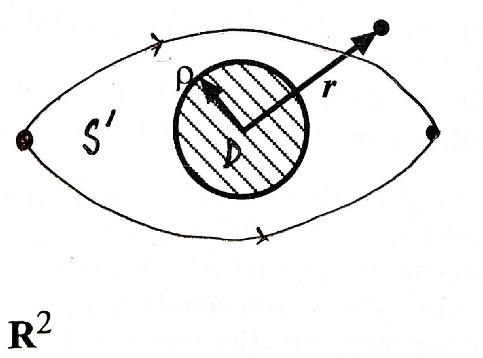
\includegraphics[scale = 0.25]{top.jpg}
\hspace{.2 in}
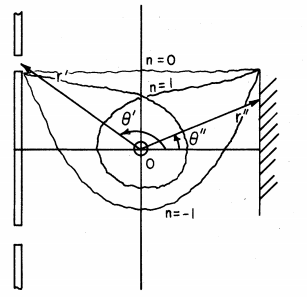
\includegraphics[scale = 0.4]{winding.png}
\caption{ a. The region of the physical space accesible to the wavefunction is NOT $\mathbb{R}^2$ since there's a hole which encompasses the interior of the solenoid \\
b. curves corresponding non-zero winding number around the excluded region}
\end{center}
\end{figure}

The argument for non-vanishing of the $\omega$ for non-trivial topology \footnote{Triviality mentions any topology to be globally isomorphic to $\mathbb{R}^n$ thus non-triviality is everything else. Interesting stuff happen there!} is as follows \cite{geop}:

From Stoke's Theorm, a line integral can be transformed to a surface integral where the line of our concern encircles the surface considered latter. Thus: 

\begin{align}{\label{fda}}
\oint_{C=\partial S}\omega = \int_{S}d\omega
\end{align}

Since the area marked in the picture is never possibly in the domain of trajectory for our system, thus the topological space of the domain of trajectory is $M = \mathbb{R}^2 / 2\pi\rho$ where $\rho$ is the radius of the solenoid in Aharonov Bohm Effect. And the trajectory of the two electron beams can be considered to have formed a closed loop in this domain, thus considering any curve $C$ encircling the cross-section of the solenoid, and with surface area $S$ in above figure, the are bounded by it can be seperated by that $S=S'+D$ where D is the area exclude from the domain. Thus \ref{fda} says 

\begin{align}{\label{fdhda}}
\int_{S}d\omega = \int_{S'}d\omega  + \int_{D}d\omega = \int_{D}d\omega 
\end{align}

Since in it is never guranteed to find get the closed forms $\omega$ to be exact within the holes of some topological space, therefore giving out some finite value around the excluded region. 
This rquires some remarks as: 

\begin{itemize}
\item the end-reulted phase strictlly depends on the topology of the domain of trajectory since the phase factor is independent of $S'$ which is the area enclosed by the curve within the accessible domain. Therefore is an equivalance class of trajectories giving out same value for geometric phase for a closed loop around the excluded region. 
One suitable explaination is \cite{pathAharonov} that if two trajectories are $Homotopically \ Equivalent$ \footnote{Given any simply-connected domain which here is only the accesible region of dynamics if two curves can be smoothly deformed from one to another by a one-to-one fasion then they are to be defined to be Homotopically Equivalent.} then the corresponding accumulation of the geometric phase would be equal. 

\item If a curve winds about the solenoid they require to be multiplied by the net winding number corresponding to the curve i.e. 

$$
\oint_{C=\partial S} \omega = (n_{+} - n_{-}) \oint _{\partial D} \omega
$$

where $n_+$ and $n_-$ indicate counterclockwise and clockwise winding number of the path.
\end{itemize}

In the literatur \cite{ab} Aharonov and Bohm showed explicitly the geometric phase factor for such set-up that has been discussed here. 
Considering an electron traversing a closed loop $C$ and subject to a magnetic field $B=\nabla \times A$ where the vector potentail and the magnetic field can be expressed in terms of differential forms following from : \ref{dafg} and with the definition of the magnetic field in as 3-vector dual to minknowskian electromagnetic field strength.

\begin{align}{\label{hehye}}
A = A_a dx^a \ \ \ \ \ \ \ \ \ \ \ \ \ F = dA = -\frac{1}{2}\epsilon_{abc} B^{a} dx^{b} \wedge dx^{c}
\end{align}

As mentioned above in this section, the introduction of electromagnetism in the lagrangian \ref{hiii} requires covariant-generalization in terms of of mechanical momentum (:= $\Pi$) thus:

\begin{align}
P \to \Pi := P - \frac{q}{c}A 
\end{align} 

Therefore the wavecfunction in coordinate representation indicates: 

\begin{align}
\braket{x|\Pi|\psi} = (i \hbar \frac{\partial }{\partial x^i}+ \frac{q}{c}A + \omega_i(x)) \psi(x)
\end{align}

This gives the physical interpretation of the $one-form \ \omega$ of our system of consideration.

Since within the dynamical region, where the configuration space is equivalent to $\mathbb{R}^3$ the one-forms might be ruled out of the equation. But not everywhere. Note that for this system, the origin of the electromagnetic potential being the solenoid itself, indicates the non-triviality of the domain, is indeed caused by the source of $A$, and also this figure transforms according to a gauge transformation as $A \to A' = A+df$, which gives one allowence to absorb the one-form within the coefficients of electromagnetic vector potential. Therefore one can indeed cosider from \ref{huhuhuhu}

\begin{align}{\label{connectinemememe}}
\omega = \frac{q}{\hbar c}A
\end{align}

Therefore considering $\psi(x)$ to be the wavefunction for non-elctromagnetic situation, the phase transformation corresponing to \ref{huha} then provides: under a closed loop:

\begin{align}{\label{abphase}}
\psi(x) \to \psi(x) \ exp (i\frac{q}{\hbar c}\oint_{C}A) \equiv \psi(x) \ exp (i\frac{q}{\hbar c}\oint_{\partial D}A)
\end{align}

Which indeed is the additional phase factor acquired in \cite{ab} but obatained by somewhat different procedure. [net winding number of the trajctory is considered to be 1 for general interference scenario]
Some remarks follow here:

\begin{itemize}
\item Since the electromagnetic potential is gauge-sensitive one can directly from the equal argument of \ref{gaugecheck} the \ref{abphase} indeed is gauge invariant.

\item Writing it in terms of field strenth dual, ie. $B$ in electromagnetism by a surface integral clears the understanding so far from \ref{hehye}: 

\begin{align}
i\frac{q}{\hbar c}\oint_{\partial D}A = i\frac{q}{\hbar c}\int_{D} dA = i\frac{q}{\hbar c}\int_{D} F^n = i\frac{q}{\hbar c}\int_{D} B .ds = i\frac{q}{\hbar c} \Phi_B  
\end{align}
\end{itemize}

Which turns out to be the magnetic flux through the surface enclosed by the trajectory of the wavefunction, which reclects in the relative phase at the inteference patters of at the screen. Therefore the key-result of this section is thus to calculate the $\textbf{Aharonov-Bohm Phase}$ which is;

\begin{align}
\gamma_{n}^{AB}(\Phi_B)= exp (i\frac{q}{\hbar c}\Phi_B  )
\end{align} 

Noting that if $\Phi_B$ is integer multiple of $\frac{2\pi q}{\hbar c}$ then the whole phase factor vanishes leaving and the fringe shift is maximum for $\Phi_B$ being half-integer times $\frac{2\pi q}{\hbar c}$. For a detailed description of the interference patters, experimental verification and other physical application of this AB effect one may refer to \cite{goodone}
\section{Geometri phase as Holonomy of Parallel Transport over U(1) Fibre Bundle:}

The mathematical richness of Geometric Phase lies in one of the its interpretations provided by B. Simons which followed the publication of M.V. Berry's Quantal Phases Accompanying Adiabatic Evolution, specifically pointing out that the Geometric Phase indeed is the holonomy of the parallel transport of the state over Parameter space with U(1) structured principal bundle over it, constructing the Hilbert space friom its eigenbasis at each point over the parameter-manifold, constituting in itself the Hilbert-fibre for say. Apparently such interpretation might sound ramification of already described (elementarlily under several conditions) mystery, but it unifies all the accountability, and properties of the Geometric Phase which gives the greater picture of this physical phenomenon. Also the usages of fibre bundles and its right-action of the structure group as Gauge-Independence was in the process of nurturing and so the ideas of fibre-bundle, its projection map, local connection one-form and parallel transport through the fibres. Even though such ideas are from Gifferential Geometry and primarily manifested in Physics throgh Einstein's introduction of Riemannian Manifold and metric-tensor field as the geometric characteristic of Gravity. Later on such great concepts were adored in greater physics community. 

For the purpose of this paper which is to present the holonomic interpretation of the geometric phase, the necessary concepts will be built and detailedly discussed. Introductorily a fibre bundle is a family of fibres, where each fibre is a manifold, say a vector space, a tensor space of whatever kind of smooth manifold one can think of. Given a smooth manifold \footnote{definitions of such aspects is provided in the appendix}, one can consider constructing at each point, a fibre. Say, for an example $S^2$ a sphere embedded in $\mathbb{R}^3$ and clearly at eact point over it, there belongs a tangent $T_p S^2 \ \forall p \in S^2$ therefore the the Tangent Bundle in this example is the disjoint union of the Tangend Spaces over manifold. In this context, every fibre itself is a vector space of namely the tangent space, thus is called in general a vector bundle. 

There exists a global $connection$ in the total space (fibres + base-manifold\footnote{Base manifold is the one over which the fibres has been constructed}) that smoothly glues together the fibres so that any information over the base manifold can be smoothly moved throughout the total space, or in other words one might say, in order to $lift$ any geometric information through the fibres precisely, one needs to have additional structure to the fibre bundles, which here is how they're $connected$. This provides rule to move $parallel$ in the total-space with respect to any given vector field over the manifold, though over a closed loop over any arbitrary curve one lands up over the fibre of the initial one for sure, but with a discrepancy, which exactly is the Holonomy associated with the connection of the fibre-bundle and curve. 

In the following subsections, the topics that will be considered are as follows; what exactly is this fibre bundle, why a $connection$ is required and why it is an one-form, horizontal lift and parallel transport of a curve and lastly the holonomy. Later on the its manifestation in describing geometric phase will be presented. Some necessary defintions to start off are provided in the Appendix. There are extraordinarily sophisticated concepts related to such this differential geometric topic regarding these but mostly necessary ones will be stated with proper care.

Throughout this section we would consider $blob$, a hypothetical character living in the total space, who can go up-down over a fibre, and left-right from fibre to fibre and can walk freely over the manifold about all its dimensional degrees of freedom. 


\subsection{Theory of Fibre Bundle: }



\begin{theorem}
A bundle (of Topological Manifolds) is a triple $(E, \pi, M)$ where $E$ and $M$ are topological manifold called the $total \ space$ and $base \ space$ respectively and $\pi$ is a continuous, surjective map $\pi: E\to M$ called the $projection \ map$
\end{theorem}

throughout this section a bundle will be denoted alternatively by $\pi : E \to M$ or by $E \overset{\pi}{\to} M$

\begin{figure}[h!]
\begin{center}
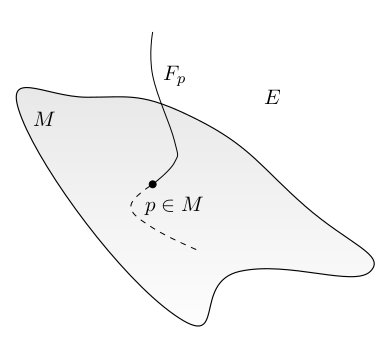
\includegraphics[scale = 0.4]{justbundle.png}
\hspace{0.2 in}
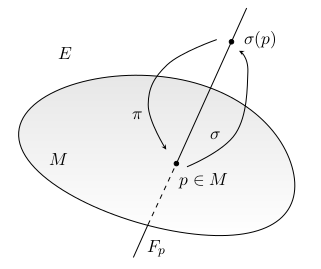
\includegraphics[scale = 0.4]{sectionmap.png}
\caption{a. \ Fibre over a point p of a base manifold M  b. \ section map $\sigma$}
\end{center}
\end{figure}

The simplest among all is the $product \ bundle$ which is, just as the name says, globally product of two topological spaces, i.e. a $Cylinder \equiv \pi : S^1 \times R^1 \to S^1$. Since such total spaces can be defined globally to be a equivalent product of two spaces, there exists a global trivialization of the total space. \footnote{A topological space is trivial if it permits one global chart}

This bundle structure can have arbitrarily anything, provided whatever it is, is well-defined. Starting from a real line-bundle ($\mathbb{R}$) over any manifold, to any continuous symmetry group can be put at each point over a manifold with suitable consideration. The total space defined $E$ is the collection of all the bundles and the manifold itself. And reference of bundle-space would mean the collection of bundles only. 

\begin{theorem}
Let $E \overset{\pi}{\to} M$ be a bundle and let $F$ be a manifold, then $E \overset{\pi}{\to} M$ is called a Fibre Bundle with typical fibre F if: 
$ \forall p \in M \ preim_{\pi}(p) \simeq F$

\end{theorem}

It is often expressed as: $F \to E \overset{\pi}{\to}M$ \footnote{Given a map $\phi: A\to B$ and $V \subseteq B = image(\phi)$ then $preim_{\phi}(V) := \{a \in A \ | \  \phi(a)=V\}$ is called the preimage of $V$ under the map $\phi$}. And the preimage of $p \in M$ under the projection map is isomorphic the bundle that is under consideration, which is F here. It is like $blob$ when walking over the base-manifold, at each point looks up or down, which is the $preim_{\pi}$ map for him, and sees each fibre is equivalent (isomorphic) to one structure, namely F. In this section, fibre at point $p \in M$ would be denoted as $F_p$


\begin{theorem} {\label{section}}
let $E \overset{\pi}{\to} M$ be a bundle with $\pi$ its projection map. A map $\sigma : M \to E$ is called a (cross-)section of the bundle if: $ \pi \circ \sigma = id_{M}$
\end{theorem}

This exactly like $blob$ going up the a fibre and just followed the path back to where he started his journey. So, $\sigma$ takes a point over the manifold and puts it somewhere on the fibre $F_p$ where the projection map takes it back over the point on the manifold thus the identity relation is defined. 

Consider a kick-start, the $Tangent-Bundle$ slightly thorough exemplary discussion:

Given a n-dimensional manifold $M$ it's tangent bundle is the family of tangent spaces at each point over the manifold and is defined as :

\begin{align}
TM := \underset{p\in M}{\cup} T_p M
\end{align}
The space $M$ is called the base-manifold of the tangent bundle $TM$.
Let $U_{\alpha} \subseteq M$ be an open set and $\phi_{\alpha}$ be a chart over it \footnote{See appendix for definition of open sets in a manifold and corresponding chart} then $\forall p \in U_{\alpha}$ the basis for $T_pM$ can be given as $(\frac{\partial }{\partial x ^1}_p, . . . ,\frac{\partial }{\partial x ^1}_{dim M}  )$ so that any vector $V_p \in T_p M$ can in coordinate basis and coefficient function be written as $V_p := V_{p}^i\frac{\partial }{\partial x ^p}_p$ where the Einstein summation convention has been used and will be such throughout this section.
Thus each tangent space at points themselves are a n dimensional vector space $\mathbb{R}^n$. Since the manifold, also locally is diffeomorphic to $\mathbb{R}^n$ the tangent spaces are exactly so and from a local-open-set point of view the total space $E$ is just $\mathbb{R}^n \times \mathbb{R}^n$. Thus there exists a map called $\textbf{local trivialization}$ which establishes a local diffeomorphism from the bundle-space from the total-space, i.e.

\begin{align}{\label{localtriv}}
    \Phi_{\alpha}:& \pi^{-1}(U_{\alpha}) \to \mathbb{R}^n \times \mathbb{R}^n \ \ \ \ \ \ \ \ \  V \to (x^1, . . ., x^{n}, V^1, . . ., V^n)
\end{align}

clearly from the definition $\pi^{-1}$ is the map that takes a point in the manifold and makes puts in somewhere over the fibre over it, and since $\pi$ is a surjective map (that it projects all the points of a single fibre to a single point on the manifold), the map $\pi^{-1}$ is a one-to-many,since its image could be any point on the fibre $F_p$ which according to this example is $T_p$.
The whole business of studying topological manifold started from Gauss's famous 1828's work, $Theorema \ Egregium$ [which indeed means the excellent theorem] which in brief says, given arbitrary 2 dimensional curved surface (namely a manifold) all its geometric properties can be studied in terms of the infinitesimal local line-segments which further generalized by Riemann to give metric tensor for general riemannain manifold as $ds^2=g_{\mu \nu}dx^{\mu}dx^{\nu}$ where $g_{\mu \nu}$ is the metric tensor field or more formally the transition functions for different patches of the manifold. In our Tangent Bundle scenario consider now a different local trivialization $\Phi_{\beta}$ defined on $U_{\beta} \in M$  such that the two open sets overlap i.e. $U_{\alpha} \cap U_{\beta} \neq \emptyset$
Therefore for some $T_p(U_{\alpha} \cap U_{\beta}) \forall p \in U_{\alpha} \cap U_{\beta}$ must be unique if it represented in terms of $U_{\alpha}$'s charts basis of that of $U_{\beta}$'s, since they must be corresponding to something identical that overlapping region, and this is where the transition functions come in and interplay between $transitions$ of different charts in the following way: 

\begin{align}
V_p = V_{p}^j \frac{\partial }{\partial x^j}_p =  {V_{p}^i}' \frac{\partial }{\partial {x^i}'}_p \implies  {V_{p}^i}'= \frac{\partial {x^i}'}{\partial x^j }_p V^{j}_p
\end{align}

Where the 2n-ordered pairs $(x^1, . . , x^n, V^1, . . ., V^n)$ and $(x'^1, . . , x'^n, V'^1, . . ., V'^n)$ are mapped by respectively $\Phi_{\alpha}$ and $\Phi_{\beta}$ as from \ref{localtriv}. 
which means for this case, in order to be able to define geometric objects as vectors, tensor, vector flows etc uniquely $\frac{\partial x'^i}{\partial x^j }$ has to be unique at every point throughout the manifold since for worst case scenario, one can consider infinite, infinitesimal overlapping regions over arbitrary manifold, but that must not matter the geometric contents over it, which also requires $det(\frac{\partial x'^i}{\partial x^j }_p) \neq 0$ otherwise everything will shrink down to a point at that corresponding overlap (such occurence raises singularity but will not be discussed further here). Also being two indices element, these $\frac{\partial x'^i}{\partial x^j }_p$ must be an element of $GL(n, \mathbb{R})$ which is the General Linear group of rank n, over the field of reals (one can consider it over the fields of complex as well but that is unnecessary for real manifold) which are $n \times n $  matrices with entries from reals. 
Therefore

\begin{align}{\label{transiboii}}
    {V^{i}_{p}}' = t_{\beta \alpha}(p)^i_j \ V^j_p \ \ \ \ \ t_{\beta \alpha}(p)^i_j = \frac{\partial x'^i}{\partial x^j }_p \ \ \ \ \ t_{\beta \alpha}(p) \in GL(n, \mathbb{R})
\end{align}

These are $\textbf{transition functions}$ which determine the $transition$ of coordinate-representation over charts to charts in their overlaps. One can readily argue how these transition functions must form a group, and the argument is as follows: 

Consider n-overlapping charts or coordinate patches of a manifold namely $U_1, U_2, .. U_n$ with each local trivialization $\Phi_1, . . ., \Phi_n$ such that $U_1 \cup . . . \cup U_n \neq \emptyset$ and say $p \in U_1 \cup . . . \cup U_n \neq \emptyset$ and from the definition of transition function, it is: $t_{12}(p)^{i}_j = \frac{\partial x^{1i}}{\partial x^{2j} }_p,  t_{23}(p)^{k}_l = \frac{\partial x^{2k}}{\partial x^{3l} }_p, . . . , t_{(n-1)n}(p)^{y}_{z} = \frac{\partial x^{1y}}{\partial x^{2z} }_p$ with which, from the composition of derivative, say ${t_{32}}^i_{j} = {\frac{\partial x^{3i}}{\partial x^{2j} }}_p = \frac{\partial x^{3i}}{\partial x^{1k}}_p \frac{\partial x^{1k}}{\partial x^{2j} }_p = {t_{31}}^{i}_k {t_{12}}^{k}_j$ which clearly verifies the group composition rule. Thus considering $S(n)$ to be the set containing all the transition functions of thus n-overlap, as $S(n) := \{ t_{12}(p), . . . .,t_{m,n}(p)\}$ (note that given n-overlap $\exists n!$ numbers of unique possible overlaps and thus transition functions which says it is just symmetry group of order n or $n\times n$ matrices) Thus considering $n=\infty$ i.e. infinite patches, it still holds, and the arguments get more general even.

\begin{theorem}
The $\textbf{Structure Group}$ of a fibre is the group of transition functions $\forall p \in M$
\end{theorem}
Therefore in this case it is $GL(n, \mathbb{R})$ . These transition functions and therefore the group of all of then determines the topological properties of the manifold since one can choose arbitrary coordinate chart and with the help of overlapping of coordinate patches one retrieves the necessary topological information of the manifold of concern, which also gives general coordinate-choice independent description of the manifold. From this point on, we would denote $G$ to be the structure group of the manifold.
That was pretty much an exemplary view but in general one must impost differentiable structures in order \ref{transiboii} to be a valid expression, therefore requires attention

$\textbf{Differentiable Fibre Bundle}$ is a structure $(E, \pi, M, F, G) $ such that: 
\begin{itemize}
\item Three manifolds $E, M, F$ are namely the $total \ space, \   base \ space, \   fibre$ 
\item  A global surjective map $\pi:E \to M$ which, including its inverse $\pi ^{-1}(p \in M):= F_p $ are smooth maps \footnote{For $\phi: A \to B$ a map is smooth if $\phi \in C^{\infty}(A)$ which is the set of infinitely-differentiable functions on $A$}
\item A Structure group $G$ which acts on $F$ as  $left \ action$  \begin{align}{\label{leftaction}}
L_g : G \times F \to F, \ \ \ \ \ \ \ \ L_g(f):= fg \ \ \ \forall f \in F, g \in G \notag
\end{align} 
\item A set of charts $(U_{\alpha}, \Phi_{\alpha})$ where ${\ U_{\alpha}}\ $ is an open covering of $M$ s.t. \begin{align}
  					\Phi_{\alpha}: \pi^{-1}(U_{\alpha}) \to   U_{\alpha} \times F, \ \ \ \ \ \ \Phi_{\alpha}(u):= (\pi(u), f), \ \ \ \ \forall \ u \in (U_{\alpha} \times F), \  \ f \in F \notag
\end{align}
\end{itemize}
which were previously define to the $local \ trivialization$ of the fibres, which are $diffeomorphisms$ such that $\pi \circ {\Phi_{\alpha}}^{-1} = pr_1 U_{\alpha}$ where $pr_1$ is the projection onto the first factor. In other words, the local trivialization map each open set of the total space into a subset of the locally defined product (this might not always be globally definable since that would mean the total space is globally a product space hence trivial) 

\begin{itemize}
\item $\forall$ pairs $U_i, U_j$ with  $U_i \cup U_j \neq \emptyset$ \begin{align}
\exists t_{ij} \in G, \ \ \ \ \ t_{ij}: U_i \cap U_j \to F,  \ \ \ \ \ t_{ij} \equiv \Phi_{i, p} \circ  {\Phi_{j, p}}^{-1}
\end{align}  
\end{itemize}
with the definition ${\Phi_{j, p}}^{-1}:={\Phi_{j}}^{-1}(p, .): F \to F_p, \ p\in U_{\alpha}$ This gives us (exactly the example with tangent space considered above) the mechanism for finding out overlap-dependent information through the transition function, which helps jumping from one coordinate-patch from another in well-defined fashion. In this way two local trivializations $\Phi_i(u)= (p, f_i), \  \Phi_i(u)= (p, f_i)$ with $p \in U_i \cap U_j$ and $u \in \pi^{-1}(p) \simeq F_q$ are related by a diffeomorphism between the respective coordinates on the fibre: 
\begin{align}{\label{amongbundles}}
(p, f_i) =  (p, \Phi_{i, p} \circ  {\Phi_{j, p}}^{-1} f_j) =  (p, t_{ij}(p)f_j)
\end{align}

as mentioned above the definition of section through $\sigma$, $\Gamma(U, E) := $ collection of smooth local section on U. Likewise $\Gamma(M, TM)$ would denote Smooth Vector fields on $m$ where $TM$ is the tangent bundle over the manifold.

The transition functions, which enable one to move from one bundle to another $f_j \ f_i = t_{ij}(p)f_j \ \forall f_i \in F_i \ f_j \in F_j$. In other words it enables one to precisely glue together the infinitesimally close bundles to one another. Which is even conversely true, if given a manifold, a fibre, and transition functions, one can then uniquely define the fibre-space over it.

$\textbf{Bundle reconstruction:}$ Given a base-manifold $M$ together with an open covering $\{U_i\}$ a typical fibre $F$ ad a set of transition functions $t_{ij}(p) \in G$. Then the entire bundle structure can be defined as :

\begin{align}
    X [\subseteq E]: \underset{i}{\cup} \ ( U_i \times F )
\end{align}
with an equivalence relation on $X$:

\begin{align}
    \{(p, f) \sim (q, g)\} \Leftrightarrow \{p=q \in  U_i \cap U_j \neq \emptyset, \ g = t_{ij}(p)f \}
\end{align}
In other words, the reconstructed bundle structure must impose equivalence structure to the geometric objects in the chart-overlapping regions, and that is why this transtion-function require to play additional structure. When $p \in U_i, \ q \in U_j, \ f \in F$ then the total space is defined as the quotient space 

\begin{align}
E = X / \sim := \{[p, f] \ \sim \}
\end{align}
Together with the global projection map $\pi: \{[p, f] \ \sim \}  \ \mapsto p$ and the local trivializations:

\begin{align}
\Phi_{i}: \pi^{-1}(U_{i}) \to   U_{i} \times F, \ \ \ \  \Phi_{i}([(p, f) \sim])=(p,f)
\end{align}
One way to summarizing last few paragraphs is that if one know how the bundle-space are held together over the base manifold, then every geometric information on it can have unique description by defining the transition functions over regarding how the open-patches are corresponded, and like if one has the base manifold,just one fibre and the possible set of transition function then one can indeed construct the bundle space uniquely. 

$\textbf{Local Frames:}$ Given a vector bundle, fibres defined at each point over the manifold is isomorphic to a vector space of same dimension, thus can $lcoally$ consider a basis set over the vector bundles.
Consider $\forall p \in U_i, \ \{ e_1, . . ., e_{k} \}$ is a basis for $F_p$ then the corresponding section \ref{section} 

\begin{align}
\sigma_{\mu} : U_i \mapsto \ \sigma_{\mu}(U_i) \subset \pi^{-1}(U_i), \ \ \ \ \sigma_{\mu}(p)= e_{\mu}(p) 
\end{align}
 Are said to be locally induced coordinate frames of $U_i$, and once local frames are defined, the associated local trivialization \ref{localtriv} comes out naturally as $\Phi_{i}: \pi^{-1}(U_{i}) \to   U_{i} \times \mathbb{R}^{dim M}, \ \ \ \ \Phi_{i}(V^{\mu} e_{\mu}(p)) = (p, \{ V^, . . ., V^{k}\}),  \ \ \ k = dim(F)$ . Clearly one can build a local trivialization when the local-frames are given to the total space, and vise versa. Now consider two sets of local frames $\{ e_{1}(p), . . ., e_k(p) \}$ and $\{ {e_{1}}'(p), . . ., {e_k}'(p) \}$ to be a local frame on the bundle over $p \in U_i \cup U_j$ Then the local change of frame is given as: 
 
 \begin{align}
 {e_{i}}'(p) = G_{i}^{j}(p) e_{j}(p), \ \ \ G_{i}^{j}(p) \in GL(dim F, \ \mathbb{R})
 \end{align}
 Thus $\forall V \in E_{p}$ with $V = V^i(p) e_{i}(p) = {V^j(p)}' {e_{j}}'(p) \implies V^i(p) = {G_{j}^{i}(p)}^{-1} {V^j(p)}'$ which also indicates ${G_{k}^{i}(p)}^{-1} {G_{j}^{k}(p)} = \delta^{i}_{j}$ which is indeed equivalent to \ref{transiboii} but with more general structure such that the fibre is not necessarily a tangent vector space, but arbitrarily anything. Upto this point I think it covers some crucially necessary idea behind a bundle over some manifold, which for physical context is once the Parameter space and in another case the Projective Hilbert Space. But the idea of Principal fibre bundle also requires greatly the notion of Lie Group and its associated Lie Algebra and how it acts on the manifold. In the following subsection, those will be mentioned.
 
 \subsection{Lie Group and Lie Algebra:}
 The theory of Lie group and its corresponding algebra is of one of the most prior interests in physics, since it precisely represents Continuous Symmetry, even from the name $group$ it suggests, by the words of mathematician John Conway, mathematically talking about symmetry, where unlike $\mathbb{Z}_n$ or their cyclic group which generally are of discrete type, the study of Lie Theory is all about continuous ones. Definitions and examples within this section and some of the following will maintain notations engaged in \cite{geomanatomy} and \cite{doeslie}
 \textbf{Lie Group:} is a group $(G, \circ)$ where $G$ is a smooth manifold and the maps 
 
 \begin{align}
     \begin{split}
         \mu:& G \times G \to G \\
         & (g_1, g_2) \mapsto g_1 \circ g_2
     \end{split} \\
     I:& G \to G \\
     & g \mapsto g^{-1}
 \end{align}
 
 Where $\circ$ is the group operation where as this is a manifold can be thought of the operation of moving around over the manifold, exemplarily similar to the addition over $\mathbb{R}^n$. And since $G$, although being a group, is manifold, $G\times G$ is indeed a globally product manifold and this inherits the atlas of the $G$. 
 
 $Example$: $S^1 := \set{z \in \mathbb{C}| |Z| = 1}$, and $(\cdot)$ be the usual complex-number multiplication operator then $(S^1, \cdot)$ is then group. This usually called $U(1)$ since it is one-parameter family of unitary operators, i.e. ever element of this group can be defined as a complex phase value, i.e. 
 
 \begin{align}
 U(1) = \set{e^{ i\gamma }| \forall \gamma \in \mathbb{R}}
 \end{align}
 
 One can readily see U(1) contains such complex numbers whose norm indeed is 1. Since $S^1$ or an usual circle in $\mathbb{R}^2$ is a simple manifold, one directly sees U(1) indeed is a Lie Group \footnote{since exponential multiplication under real argument is abelian i.e. $e^{ i\gamma_1} \cdot e^{ i\gamma_2} = e^{ i(\gamma_1+\gamma_2)} \ \forall  \gamma_1, \gamma_2 \in \mathbb{R}$}. This is the key ingredient of our understating of the phase factors associated to be an element of $U(1)$ which one can construct to be a fibre bundle over the projective Hilbert Space, and will be nurtured in the following sections.
 
$ \textbf{Definition}$ Let $(G, \sbullet)$ and $(H, \sbullet)$ be Lie Groups. A map $\phi : G \to H$ is a $Lie \ Group \ homomorphism$ if it is a Group homomorphism\footnote{A homomorphism between two groups preserves the necessary algebraic structure and the domain-group can be embedded into the image one, please see Appendix for more on this} and a smooth map. A Lie group homomorphism is a group homomorphism which is also a diffeomorphism \footnote{a diffeomorphism is an isomorphism of manifolds}.
 
 Given the lie group it must be mentioned possible ways it can act on itself, considering the general non-abelian case it must be seperated to be a $left-action$ and a $right action$ over its elements. \footnote{whatever definition is provided here regarding left-action of the lie group, is equivalent to the right-one, they are in general considered seperated to make sure the general non-commutative structure of the group, but in our purpose where U(1) is the lie group, which is commutative, it won't matter} 
 
 $\textbf{Definition}$: Let $(G, \sbullet)$ be a lie group and consider $g \in G$ and element. The map 
 
 \begin{align}
     l_g:&  G \to G \notag\\
     & h \in G \mapsto l_g(h) := g \sbullet h = gh  
 \end{align}
 which is just usual group operation from the left; and can be thought of as a $left \ translation$ and the group operation notation has been suppressed and will in general be so throughout the section. Since $G$ also is smooth manifold, it must have necessary differential structure embedded in itself, therefore geometric objects like vectors, covectors, tensors of arbitrary kind must also be well-defined throughout, which requires more ideas here. 
 
 \textbf{Proposition:} Let $G$ be a lie group then $\forall g \in G$ the left-translation map $l_g:  G \to G$ is a diffeomorphism.
 
$proof:$ Let $h, h' \in G$ Then we have 
\begin{align}
    l_g(h) = l_g(h') \Leftrightarrow gh = gh' \Leftrightarrow h = h'
\end{align}
moreover $\forall h \in G, \ \exists g^{-1}h \in G$ and 

\begin{align}
    l_g(g^{-1}h) = g g^{-1} h = h
\end{align}
 Therefore, the operation $l_g$ over $G$ is a bijection on $G$. Note that: $l_g = \mu(g, _ ))$, and since $\mu: G \times G \to G$ is a smooth by definition, so is $l_g$. The inverse map is ${(l_g)}^{-1}=l_{g^{-1}}$ since:
 
 \begin{align}
     l_{g^{-1}} \circ l_{g} =  l_{g}  \circ l_{g^{-1}} 
 \end{align}
 Then for the same reason as above with $g$ replaces by $g^{-1}$ the inverse map ${(l_g)}^{-1}$ is also smooth. Hence the map $l_g$ is indeed a diffeomorphism.  
 \[
\pushQED{\qed} \qedhere
\popQED
\]  
 
 Since the map $l_g$ is a diffeomorphism over the manifold $M$ its pushforward and pullbacks can be thus defined to map smooth-vector fields from its domain's tangent bundle to smooth vector fields over the image's tangent-bundle, obviously within $G$, likewise covectors, or even n-differential forms can be pulled back from the cotangent-bundle of the image to the cotangent-bundle of the domain. Namely the differential properties can be played around since $l_g$ is a diffeomorphism.  The push-forward \footnote{See appendix for definition of push-forward map induced by some map} map induced by the left-translation is as:
 
 \begin{align}{\label{fafdfsd}}
     {l_g}_{*} :& T_hG \to T_{l_g(h)}G = T_{gh}G  \ \ \ \ \forall h \in G \notag \\ 
     & X \mapsto {(l_g)}_{*}(X) \notag
     \end{align}
where $ {(l_g)}_{*}(X) : G \to TG $ namely $X$ belongs in the family of vector fields, its pushforward also is a family of vector field, thus its image is the tangent bundle of $G$. Now from the first expression the pushforward map is defined pointwise from tangent space of one point to another over the manifold.

Since the pushforward of the left-translation map \footnote{pushforward of a map is only well defined throughout a manifold when the map itself it a diffeomorphism which is why the diffeomorphism of $l_g$ has been proved previously} has been introduces, the left-invariant vector fields can thus be stated noting that, this constructs the Lie-Algebra of the corresponding Lie-Group.  If defined pointwise, the pushforward map of $l_g$ turns out ${({(l_g)}_{*}(X))}_{h} = {(l_g)}_{*}(X)_{g^{-1}h}$ Since from \ref{fafdfsd}$X \in T_hG$ and ${(l_g)}_{*}(X) \in T_{gh}G$ therefore under left-translation map, in order for a vector field to be same somewhere under its pushforward, pointwise speaking it must start from inverse-left-translated point over the manifold.

\textbf{Definition:} Let $G$ be a Lie group. A Vector Field $X \in \Gamma(TG)$ is said to be $left-invariant$ if

\begin{align}
    \forall g \in G : {(l_g)}_{*}(X) = X
\end{align}
Equivalently this hold pointwise if one writes: [from \ref{fafdfsd}] 

\begin{align}{\label{boom}}
\forall g, h \in G: {(l_g)}_{*}(X_h)=X_{gh} 
\end{align}
 by calling the definition of pushforward again we have $X \in \Gamma(TG)$ is left-invariant (or more-precisely, invariant under pushforward of left-translation) if and only if:
 
 \begin{align}{\label{dagdsbdz}}
 \forall f \in C^{\infty}(G): X(f \circ l_g) = X(f) \circ l_g
 \end{align}
 It is defined in the literature (just notationally) the set of all left-invariant vector fields over the lie group $G$ as $\mathfrak{X}(G)$ and clearly $\mathfrak{X}(G) \subseteq \Gamma(TG)$\footnote{again $\Gamma(TG)$ is the set of vector fields over $G$ or namely the collection of elements of $G$'s tangent bundle} . Some significant property of the $\mathfrak{X}(G)$ is that it is closed under addition\footnote{the addition here defined is for elements in $T_hG$ for some $h\in G$ i.e. standard vector space addition since $T_hG \simeq_{isom} V$}. And this collection of left-invariant vector-spaces have some significant properties which will be stated and proved hereafter. 
 
 $\mathfrak{X}(G)$ is closed under addition between two of its elements and also closed under multiplication with a $f \in C^{\infty}(G)$ i.e.
 
 \begin{align}
    \begin{split}
        \textbf{+} : \mathfrak{X}(G) \times\mathfrak{X}(G) \to \mathfrak{X}(G) \notag 
     \end{split}\\
    \begin{split}
        \sbullet[.75]  : C^{\infty}(G)\times \mathfrak{X}(G) \to \mathfrak{X}(G) \nonumber
    \end{split}
\end{align}

$proof:$ 1) Take, $X_1, X_2 \in \mathfrak{X}(G)$ therefore from the definition of ${(l_g)}_{*}$ \ref{boom}      ${({(l_g)}_{*}(X_1) )}_{h}= {(X_1)}_{gh}$ and ${(l_g)}_{*}$ \ref{boom}      ${({(l_g)}_{*}(X_2) )}_{h}= {(X_2)}_{gh}$
 and since ${(l_g)}_{*}(X_1 + X_2) = {(l_g)}_{*}(X_1)+ {(l_g)}_{*}(X_2)$ \footnote{as maps of ${(l_g)}_{*}$ is from a vector space to a vector space in linear fashion, and the pushforward is often regarded in literature to be differential map of a map which is $l_g$ here} Thus: ${(l_g)}_{*}(X_1 + X_2) = X_1 + X_2$ which is true $\forall X_1, X_2 \in \mathfrak{X}(G)$ 
 2)  Take $X\in \mathfrak{X}(G)$ and $f \in C^{\infty}(G)$ and from \ref{boom} and \ref{dagdsbdz} ${{(l_g)}_{*}(f \sbullet[.75]   X ) }_{h}= {(f \sbullet[.75]   X)}_{l_g (h)} = f_{gh} X_{gh}$ \footnote{since pointwise any function and a vector-field is just a number and can be multiplied directly}
  \[
\pushQED{\qed} \qedhere
\popQED
\]  
 
 Therefore these elemets of $\mathfrak{X}(G)$ are special interest as they are closed under basic operations, and also vector fields over group-structured manifold. Among many other significant properties of it, is that $\mathfrak{X(G)}$ is a vector space isomorphism with respect to $T_eG$ where $e = id_{G}$\footnote{the proof is not presented here but one can find it in \cite{geomanatomy} or \cite{doeslie}}
 
 But in order to move further and talk about Lie-Algebra generated by the Lie Group, the general perspective of an algebra needs to be mentioned which is as follows: 
 
 $\textbf{Definition:}$ Given a vector space $V$ over a field $F$, an Algebra over $V$ is the vector space equipped with a billiear map 
 
 \begin{align}
     whatever:& V \otimes V \to V \\
     & (v_1, v_2) \mapsto v 
 \end{align}
 Thus $(V, Whatever)$ is then an algebra. For our regular correspondence, the $V$ is $\mathbb{R}$ and $whatever = +$ of addition of reals. An algebra could be associative or non-associative, and the latter one will be the case for Lie Algebra. 
 
 
 $\textbf{Definition}$ A Lie Algebra $(\mathfrak{X}(G), +, \sbullet[.75] A, [\![ . \ , \ . ]\!])$ is a $k=dim(\mathfrak{X}(G))$ vector space equipped with the operation $[\![ . \ , \ . ]\!]$ such that
\begin{itemize}
\item Bilinear: $[\![ . \ , \ . ]\!] : \mathfrak{X}(G) \times \mathfrak{X}(G) \to \mathfrak{X}(G)$
\item Skew-Symmetric: $[\![ x \ , \ .y]\!] = - [\![ y \ , \ x ]\!]  \ \ \forall x, y \in \mathfrak{X}(G) $
\item Respects Jacobi's Identity: $[\![ x \ , \ [\![ y \ , \ z ]\!]  ]\!] +[\![ y \ , \  [\![ z \ , \ x]\!] ]\!] +[\![ z \ , \ [\![ x\ , \ y ]\!]  ]\!] =0 \ \ \ \ \forall x, y, z \in \mathfrak{X}(G)$ 
\end{itemize} 
  But it requires a proof that indeed the the result indeed is an element of $\mathfrak{X}(G)$ under the operation $[\![ . \ , \ . ]\!] $ and it is, by its action is defined as: 
  
  \begin{align}
  [\![ X \ , \ Y ]\!](f) := X(Y(f)) - Y(X(f)) \ \ \ \  \forall x, y \in \mathfrak{X}(G) \ and \ \forall f \in C^{\infty}(G)
  \end{align}
  
  $\textbf{statement:}$ $\forall X, Y \in \mathfrak{X}(G) \implies [\![ X \ , \ Y ]\!] \ \in \mathfrak{X}(G)$ 
  
  $proof:$ $\forall g \in G \ $and $f \in C^{\infty}(G) \ $we have: 
  \begin{align}
  [\![ X \ , \ Y ]\!](f \circ l_g) &=X(Y(f \circ l_g)) - Y(X(f \circ l_g ))  = X(Y(f) \circ l_g ) - Y(X(f) \circ l_g ) \\
  & = X(Y(f)) \circ l_g - Y(X(f)) \circ l_g  = \{ X(Y(f)) - Y(X(f))\} \circ l_g =   [\![ X \ , \ Y ]\!](f)  \circ l_g
  \end{align}
 Therefore from the definition \ref{dagdsbdz} it says indeed $[\![ X \ , \ Y ]\!] \ \in \mathfrak{X}(G)$
 
   \[
\pushQED{\qed} \qedhere
\popQED
\]  

Lastly in this subsection a brief identification of the $exponential \ map$ which retrieves locally the $Lie \ Group$ elements from its left invariant vector fields or the $Lie \ Algebra$, and the idea of $Adjoint \ map$ will also be briefly sketched since these all will be essential in talking about Principal Fibre Bundle and correspondingly the Connection one-form over the bundle space, which will turn out to be $Lie \ Algebra \ Valued \ one \ form.$ Since a lie algebra can be formed from any vector space, provided they have built in the so-called $commutator \ bracket$. But one can in other way as well construct the Lie group from the Lie Algebra (upto local diffeomorphism). Although this process yeilds a $one-parameter \ subgroup$ of the bigger lie-group, it nevertheless satisfies our necessity since $U(1)$ the group itself is a $one-parameter \ group$ and thus it can be totally retreied by its corresponding $Lie \ Algebra$. \footnote{the proof here is sketched shortly and one can find that in lec18 of \ref{geomanatomy}}

$\textbf{Theorem:}${\label{lieidentan}} $\mathfrak{X}(G) \simeq T_eG$ \footnote{it is vector space isomorphism since both are so}

$proof:$ We have $X_e \in T_eG \ e = id_{G}$ now define a vector fielf $L^X = {(l_g)}_{*}(X) \ \forall g \in G$ which is the pushforward of the vector $X$ at each point over the manifold by evaluated by left-translation. thus

\begin{align}
{(l_g')}_{*}(L^x) = {(l_g')}_{*}({(l_g)}_{*}(X)) = {(l_{g'g})}_{*}(X) = L^{X}_{g'g} \in \mathfrak{X}(G) \  \ \ \forall g, g' \in G
\end{align}
which says every vector field generated by pushforward of left translation from elements of $T_g$ are left invariant vector fields since \footnote{for two diffeomorphisms ${(l_g')} and {(l_g)}$ one can write $({(l_g')}_{*}({(l_g)}_{*}v)) = {({(l_g')} \circ  {(l_g)})}_{*}v$}{\label{ndfushdofsd}}. and now the converse requires attention. 
$\forall Y \in \mathfrak{X}(G)$ by definition ${({(l_g)}_{*}(Y))}_{h}={(l_g)}_{*}Y_{gh}$ thus for some vector field $Y$ at some position $h\in G$ one can take it back to the $e \in G$ smoothly that

\begin{align}
{{(l_{h^{-1}})}_{*}(Y))}_{h}= Y_{ {h^{-1}} h} = Y_{e}\in T_{e}G \ \ \forall h, g \in G 
\end{align}
Which says every $ Y \in \mathfrak{X}(G)$ can be made an element of $T_{e}G$ Therefore  $\mathfrak{X}(G)$ and $T_eG$ has good one-to-one correspondence.   \footnote{that's a very crude way to present the proof, one can find well elaborated one here \href{http://bose.res.in/~amitabha/diffgeom/chap21.pdf}{link}}
   \[
\pushQED{\qed} \qedhere
\popQED
\]  

One can further see $(\mathfrak{X}(G), [\![ . \ , \ . ]\!])$ and $(T_eG, [. \ , \ .])$ are equivalent where the latter is regular commutator bracket for $T_eG$ elements.

Therefore further on we can consider any element from $\mathfrak{X}(G)$ to be from $T_eG$

$\textbf{Definition:}$ Let $G$ be a lie group, and let $A \in T_eG$ then the map

\begin{align}{\label{exponentialmap}}
    \zeta^{A}:& \mathbb{R} \to G, \  \ \ \ \  \lambda \mapsto \zeta^{A}(\lambda) := exp(\lambda A)
\end{align}

is a $\textbf{One Parameter Subgroup}$ of $G$. One can readily see this well-defined $\forall \lambda \in \mathbb{R}$ and for $A \in T_eG \simeq \mathfrak{X}(G)$ image of the map $\zeta^{A}$ is an element of the Lie Group $G$. \footnote{The choice of the function to be $exp$ is necessarily to ensure the group sructure of the $G$ since exponential maps form groups, and they are smooth, also for arbitrary matrices as well, it can be provided as power series expansion which indeed is converging for any metric space, which $\mathbb{R}$ clearly has}

$Example$  \textbf{U(1) Lie Group}: For the Lie Group to be $S^1 \simeq U(1)$ one can directly see its tangent space is a real line, and so at the origin we definitely have: $T_e(U(1)) \simeq \mathbb{R}$ and considering a map 
\begin{align}
    \bar{i}:&  \mathbb{R} \to \mathbb{C} \\
    & r \mapsto ir \ \ \ \ \ \ i = \sqrt{-1}
\end{align}

it is just every number of $\mathbb{R}$ is multiplied by $i$ and clearly this is a diffeomorphism of $\mathbb{R}$ since it respects the manifold structure of $\mathbb{R}$ and the maps $\bar{i}$ and $\bar{i}^{-1}$ are both smooth. thus $\mathbb{R} \simeq \bar{i}(\mathbb{R})$ Therefore the Lie Algebra associated with $U(1)$ is just $\mathbb{R}$ indeed the simplest case possible and therefore the group element are taken from exponentiating elements from real-line (definitely an $i$ required to catch up with Euler's identity) 

\begin{align}
U(1) = \set{ exp(\lambda) |  \lambda \in \bar{i}(\mathbb{R}) \simeq \mathbb{R}}
\end{align}

Lie groups are in general represented as a map from the group to a General Linear group over some vector space ie. $R: G \to GL(V)$ where V is some vector space, and being linear, this forms a representation of the corresponding Lie Group. Now given a Lie group, one can immidiately construct the Lie Group, and therefore the $V$ of our concern can be $\mathfrak{X}(G)$ or the Lie-Algebra itself, which is nothing  but the Tangent Vector Space at the origin. One such map is $Adjoint \ Repsentation$ of a Lie Group which has some interesting properties and will be used in developing ideas of $Connection \ one \ form$ over Principal Fibre Bundles and correspondingly its holonomy associated with the parallel transport with respect to the connection over the total space.

$\textbf{Definition:}$ Let $G$ be a Lie Group. 

\begin{align}
    \forall g \in G \ \ \ \ \ Ad_g :& G \to G \\ 
    & h \mapsto g h g^{-1}
\end{align}
Is called the Adjoint map of the Lie Group, and since it is a compostion of Lie Group operation and each element themselves are smooth, it smooth as well and also its inverse is smooth. Moreover one has 

\begin{align}
    Ad_g(e) = geg^{1} = gg^{-1} = e
\end{align}
which simply maps the identity of the group to the identity only. Therefore $pushforward$ of this map will be ${Ad_{g}}_{*}: T_hG \to T_{{Ad_{g}(h)}}G \equiv   T_{(ghg^{-1})}G${\label{adjointmap}} which readily indicates ${Ad_{g}}_{*}(e): T_{e}G \to T_{e}G$ i.e. this map, maps Lie-Alegbra elements to themselves, as \ref{lieidentan}. Therefore considering the map $Ad: G \to GL(T_eG)$ such that $Ad: g \mapsto {Ad_g}_{*}$ which indeed defines a representation of the Lie Group. 

It's suitable to end this subsection by noting that there is an extensive study in the text-materials regarding the concepts just mentioned and briefly proved here, and only the handful ideas regading those has been presented which seems necessary regarding studying the mathematics underlying the Geometric Phase.

\subsection{Principal Fibre Bundle}
Principal Fibre Bundles are fibre bundles whose typical fibre is a lie group, and this makes them one of the few uttermost beasts, since its its bundles are each a manifold and also a group. It requires a proper notion not only how the fibres are constructed but also how the group $acts$ on the total space. This allows the understanding of any fibre bundle on which the Lie Group $acts$. These are often called $Associated \ Fibre \ Bundles$ and will be mentioned later on. Notations here as well follow

$\textbf{Definition.}$ Let $G$ be a lie group and let $M$ be a smooth manifold. A smooth map

\begin{align}{\label{rightaction}}
\vartriangleright  \ :&  \ G \times M \to M \\ 
& (g, p) \mapsto R_g(p) := p g 
\end{align}
is called the Right Action\footnote{the operation $\vartriangleright$ in general is no meaning unless some representation of the Lie group has been provided, i.e. if $R : G \to GL(V)$ be a representation of $G$ on a vector space $V$ then $\vartriangleright$ would correspond to right action of the corresponding representation $R_g$ on elements of the manifold} of $G$ on $M$. It is equivalent for $Left-Action$. \footnote{It these contexts the left and right actions are seperated to make sure the Lie Group might not be Abelian in general, but if one Lie Group is indeed Abelian, these right and left action won't matter as for the case of $U(1)$ right and left actions are equivalent.}

$\textbf{Definition:}$ Let $G$ be a Lie Group. A smooth bundle $(E, \pi, M)$ is called $Principal$ $G-bundle$ if $E$ is equipped with a $right$ $G-action$ such that:

\begin{align}{\label{principalfibrebundledefinition}}
E \overset{\pi}{\to} M  \ \ \simeq_{bdl} E \overset{\rho}{\to} E /G
\end{align}
Where $\rho$ is the quotient map, defined by sending each $p \in E$ to its equivalence class (i.e. orbits) in the orbit space $E/G$. This requires slight elaboration and is as follows: The orbit space for our map $\vartriangleright  \ : \ G \times M \to M $ is defined as:

\begin{align}
\begin{split} {\label{osfdspg}}
G_p : = \{	q \in M	| \exists g\in G \ : q = g \vartriangleright  p \}
\end{split}\\
M/G := M/ \sim = \{G_p | p\in M \}
\end{align}
Or in other words, $G_p$ is the collection of points over the manifold, from a perticular point $p$, where I can go, with the action of all the elements of the group $G$. In is named as $Orbit$ of the point $p$. And likewise, $M/G$ is the collection of orbits of the all points over the manifold that has been formed by the equivalence class of all the elements of the group's action on the points. It was mentioned before regarding bundles in general that locally the total space looks like a product space, i.e. in this case for an open chart $U_i \subseteq M  \  \ \exists \sigma: U_i \to U_i \times G \simeq E_p$ therefore considering the map from $E$ to its quotient space $\rho: E \to E/G \simeq M$  is then just equivalent\footnote{the equivalence here is according to bundle morphism which is diffeomorhism of the base space as well as the bundle-structure, which indeed is  true} to the usual budle-projection map $\pi: E \to M$. 

Therefore from the definition of this equivalence class here, it is evident that the $right-action$ is $fibre-preserving$ that is, from a point over a fibre, if I project down on the base manifold by the projection map $\pi$ then it will be equivalent to projecting another point over the same fibre, where I went with the right action of G, i.e. $\pi(u)=\pi(u \vartriangleright g) \in M \  \ \forall g \in G$. The orbit space defined by \ref{osfdspg} is just another way of considering the definition of each fibre, from just the above argument. 

Further consider a local trivialization like mentioned in \ref{localtriv}

\begin{align}
\Phi_i: \pi^{-1}(U_i) \to U_i \times G,  \ \ \ \ \ u \mapsto (\pi(u), \phi(u)) = (p, h_i)
\end{align}
\footnote{from the local trivialization, $\phi$ is such a map that assigns an arbitrary group element to the the trivialization map $\Phi_i$ such equivalence classes of the such elements will act on the fibre-points in such a way that they project over the same point} The right action on $\pi^{-1}(U_i)$ is defined as:
\begin{align}
& \Phi_i(u \vartriangleright  g) = (\pi(u  \vartriangleright g), \phi(u  \vartriangleright g)) \equiv (p, h_i g) \\
& \implies {\Phi_i}^{-1}(p, h_i  \vartriangleright g) = ug = {\Phi_i}^{-1}(p, h_i)  \vartriangleright g \ \ \ \forall u \in \pi^{-1}(U_i)
\end{align}

More exotic discussion will not be followed in this section as delving into one aspect would require exquisite discussion of some other since it being a vast notion, of which, all will not be of very usage in this purpose of this paper and we will move towards further notions.

$\textbf{Associated Fibre Bundles:}$ An associated fibre bundle is such that is associated (in a certain sense) to a Principal G bundle. In general given a Principal Fibre Bundle one can construct a Vector Bundles associated with it, over the which the Lie Group acts through its left-action. The basic idea is the following, given a principal bundle one can, from its inherent structure, contruct another bundle space. 

$\textbf{Definition:}$ Let $(P, \pi, M)$ be a Principal G-Bundle and let $F$ be a smooth manifold equipped with a left-G Action $\vartriangleleft$ such that
$P_F := (P \times F) / \sim_G$ where $\sim_G$ is the equivalence relation as:

\begin{align}
(p,f) \sim_G (p', f') : \Leftrightarrow \ \exists g\in G : p' = p \vartriangleleft g \equiv pg, \ f' = g^{-1} \vartriangleright f \equiv g^{-1}f \ \ \ p, p' \in P, \ f, f' \in F
\end{align}
And the points on $P_F$ are denotes as $[p,f]$ since they constitute this equivalence class, and 
the map

\begin{align}
\pi_{F}:& P_F \to M \\ 
& [p,f] \mapsto \pi(p)
\end{align}
which is well defined since if $[p', f'] = [p, f]$, then for some $g \in G$
\begin{align}
\pi_F([p', f']) = \pi_F([p \vartriangleleft g, g^{1} \vartriangleright f]) = \pi(p \vartriangleleft  g) =: \pi_{F}([p, f])
\end{align}

and one can directly show this is an equivalence relation \footnote{a relation is an equivalence relation if it is Reflexive, Symmetric and Transitive, which in case readily is}. The $Associated \ Bundle$ (to $(P, \pi, M)$ and $F$) is the Bundle $(P_F, \pi_F, M)$.

One can consider open coverings of $M$ and construct local trivializations over it as, for $U, V \subseteq M$ such that $U \cap V \neq \emptyset$ and $t \in U \cap V$, so local trivialization over subcoverings are in general defined as

\begin{align}
\Psi_1 :& \pi^{-1}(U) \to U \times F \\ 
& u  \mapsto (\pi(u), \phi(p)) = (p, h_U \in F) 
\end{align}
and 
\begin{align}
\Psi_2 :&  \pi^{-1}(V) \to V \times F \simeq U \times F\\ 
& p \mapsto (\pi(u), \phi(p)) = (p, h_V \in F) 
\end{align}
therefore for the overlapping region: 

\begin{align}
(p, h_u) = (p, (\Psi_1^{-1} \circ \Psi_2 )h_v) = (p, \Psi_{UV}(p)h_v)
\end{align}
Therefore one can consider covering the whole base-manifold with charts represented as $U_i$s and look for the transition functions in the overlappings and thus construct a maximal chart overlapp or namely an $atlas$ of the manifold. Note that in the above expressions F the typical fibre of our fibre bundle of concern, and it will be changed to $G$ for principal fibre bundle since in that case a typical fibre is a Lie group $G$. But then elements from the lie group will be noted from ano another by either left-translation (for associated fibre bundles) or by right-translation (for principal fibre bundles) therefore the transition functions, in some linear $GL(V)$ representation of the Lie Group:

\begin{align}
\Psi_i \circ \Psi^{-1}_j := g_{ij}
\end{align}
which one can readily identify to be the metric tensor from general relativity. Therefore in short, diagramatically representing the developement so far is according to next figure. 

\begin{figure}[h!]
\begin{center}
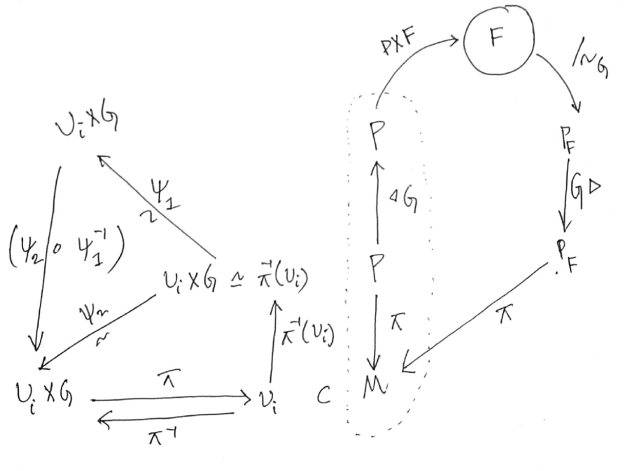
\includegraphics[
scale = 0.3]{diagram1.png}
\caption{transition map of local trivializations and associated fibre bundle structure from Lie-group fibred Principal Fibre Bundle}
\end{center}
\end{figure}

In the following subsections, connection one-form over the pricipal fibre bundle will be considered and later on horizontal lift, and parallel transport will be discussed in a bit.


\subsection{Connection:}
Even though the fibre bundles has been constructed and has been associated with other bundle structures namely the associated fibre bundles, but in order to talk precisely about measurements and they are all related over the manifold one requires intrinsic definition of how how the bundles are $connected$. We have from out regular understanding of differentiation in euclidean analysis that (for simple 1d case:) $f' = \underset{|x-y|\to 0}{lim} \frac{f(y)- f(x)}{y-x}$ which is just change of some funcion over its infinitesimal domain. Now if one wants to differentiate a function over some manifold how does one do that ? one must know the difference between values of a function over two function and also the subtraction cannot be arbitary since the manifold might not in general be $\mathbb{R}^n$ . Also differentiation might not be for a function, rather any mathematical object, like a vector. Therefore one requires a precise method to compare two of its kind, in two different points over the manifold. 

Consider one wants to compare two vectors at two points, one cannot just subtract the value of its components from two points, since these values of the components depend on the choice of chart, which might not be uniform throughout the manifold. Therefore if one knows how the manifold has changed between the points over which our comparing vectors are sitting, then one can move a vector the other point, and then measure the two as they now belong to the same tangent-space to the manifold. This is the key idea behind parallel transport of vectors over a manifold. In order to parallely move one vector with respect to itself over infinitesimally previous point, one requires the knowledge how exactly the $tangent \ spaces$ are $connected$ or $glued \ together$ over  the manifold, which in turn depends on the structure of the manifold. 
\begin{figure}[h!]{\label{dsfjsjddfkdg}}
\begin{center}
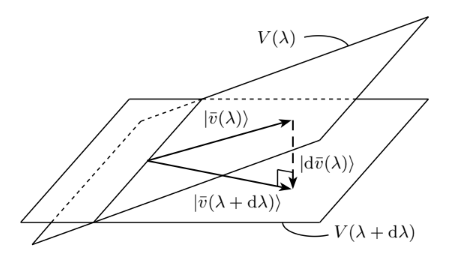
\includegraphics[
scale = 0.3]{connectiononeform.png}
\caption{connetion as one form!}
\end{center}
\end{figure}
Now there's the key idea, consider from the above diagram someone is moving the tangent space $V(\lambda)$ to infinitesimally neighbouring tangent space $V(\lambda + d\lambda )$ along the direction it wants to go and compare, where every vector on $V(\lambda)$ is orthogonally projected \footnote{one can see for infinitesimal distances, orthogonal projections are indeed parallel since some portion of the two tangent spaces are intersected so there's no possibility that any vector on $V(\lambda + d\lambda )$ will be parallel to $V(\lambda )$ and orthogonal projection is the only way out}over to $V(\lambda + d\lambda )$ and the change in the $vector \ spaces$ are indeed in the direction of a $covector$ since considering the $cotangent \ space$ the change $d \vec{v}(\lambda)$ would lie there. Therefore the change in the vector spaces themselves are related to a $covector$, thus if one knows the proper description of the covectors throughout the manifold, one can then move-parallely from point to point, and do precise measurements over the manifold. \footnote{
why not consider change of $covector-space$ and talk about connection $vectors$, well that's simply because $vectors$ are more $geometric$ than $covectors$ since covectors are linear transformations from vectors to the cooresponding fields of the vector space, one can do the converse, and do the whole, no problem! but must maintain it throughout.}And since a covector is equivalently a differential $one \ form$, the connection we must consider is an indeed called as $\textbf{connection one form}$. 

One way to talk about $connection \ one \ form$ is through considering the tangent bundle over the manifold is decomposed pointwise on its Vertical and and Horizontal part, i.e.

\begin{align}
T_pP: = V_pP \oplus H_pP
\end{align}
from the idea itself it's clear that whatever solely lives on the $vertical$ subspace of the total tangent space will be projected to the null-vector over the manifold, i.e. $\forall v \in V_pP, \ \pi(v)=0$ which is the natural projection map over the manifold from the bundle space. Therefore the $parallel \ transport$ can be thought of an assigning a collection of specifly selected $horizontal \ spaces$ such that any vector living there projects down to exacly same form, without difformation. But it is equivalent to consider a global one form over the total-space, and will consider this approach, since it will be useful in later developements. 

Let $(P, \pi, M)$ be a principal G bundle and since every element $A \in T_eG \simeq \mathfrak{X}(G)$ gives rise to a left invariant vector field on $G$ which one denotes with $X^A$ being the left invariant vector field generated by the lie algebra element $A$ as of \ref{exponentialmap}. Thus $\forall A \in T_eG \exists X^A \in \Gamma (TP)$ as
\begin{align}
X^A_p :& C^{\infty} \to \mathbb{R} \\ 
& f \mapsto \frac{d}{dt}[f(p \vartriangleleft exp(tA))] (0)
\end{align}
Where\footnote{since a vector field eats a function at each point giving out  a real number output for the field of the vector space being $\mathbb{R}$} the and derivative is taken w.r.t. the real parameter $t$ and with $\gamma(0)=p$ since the lie algebra lies over $T_eG$. 

 \footnote{denoting $X_{\gamma, \ p}$ as a vector field of a curve $\gamma (t): t \in [0,1] \to M$ with $\gamma(m)=p$ one has $X_{\gamma, \  p}(f) = (f \circ \gamma)'(m)$  by definition of vector field where the derivation is with respect to the curve's parameter} 
 
 Also define a map:
 
 \begin{align}
     i_p:& T_eG \to T_gG \\ 
     & A \mapsto X^A_g
 \end{align}
 
 $\textbf{Definition}:$ Let $(P, \pi, M)$ be a principal bundle and let $p \in P$. The vertical subspsace at $p$ is the vector subspace of $T_pP $ given by:
 
 \begin{align}
 V_pP:=& ker({{( \pi)}_{*}}_p) \\ 
 & = \{ X_p \in T_pP | {{{( \pi)}_{*}}_p(X_p)=0} \}
 \end{align}
 which are just formal way of waying that anything that lives in the vertical subspace must project down to null, but since $\pi$ maps points from total space to the points over the manifold, we must consider the corresponding pushforward. 
 
 $\textbf{lemma:}$ $\forall A \in T_eG, \ p\in P, \ \ \ X^A_p \in V_pP $ 
 $proof:$ since the action os $G$ simply permutes the elements within the fibre one has, from the exponential map from Lie Algebra to Lie Group from \ref{exponentialmap} noting that right action of $G$ over principal fibres are fibre preserving:
 
 \begin{align}
 \pi(p) = \pi(p \vartriangleleft exp(tA)), \ \ \ \ \forall t \in \mathbb{R}
 \end{align}
 Now for some $t$ let $f \in C^{\infty}(M)$ be arbitrary, then:
 
 \begin{align}
 {({\pi}_{*})}_p X^A_p (f) &= X^A_p(f \circ \pi) \\ 
 &= [(f \circ \pi)(p \vartriangleleft exp(tA))]'(0) \\
 &= [f(\pi(p))]'(0) = 0
  \end{align}
since $\pi(p) \in M$ is a fixed point thus $\forall f, \ f(\pi(p))$ has a fixed value.

This gives a significant idea, that whatever lies in the vertical subspace, are vector fields created over the whole Lie Group generated by the Lie Algebra, therefore, also it was pointed out from \ref{dsfjsjddfkdg} that the changes in the tangent spaces are indeed a member of one-form, which from the last proved lemma, must be $lie \ algebra \ valued$ \footnote{a covector sends a vector to reals, only when the vector spaces are constructed by the field of reals, in this context, the vector fields over the total space are generated by Lie Algebra, which makes it essential for the connection one form to be Lie Algebra Valued}. 

$\textbf{Definition:}$ A $Connection$ on a principal G-bundle $(P, \pi, M)$ is a choice of horizontal space at each $p\in P$ such that

i) $\forall g \in G, p\in P$ and $X_p, \in H_pP$ we have:

\begin{align}
{(\vartriangleleft g)}_{*}X_p \in H_{p \vartriangleleft g}P
\end{align}
where ${(\vartriangleleft g)}_{*}$ is the pushforward of the right-translation map

ii) for every smooth $X \in \Gamma(TP)$, there is a unque pointwise decomposition

\begin{align}
X_p = hor(X_p) + ver(X_p)
\end{align}

at each $p \in P$ which can be extended for smooth vector fields as $hor(X),ver (X) \forall X \in \Gamma(TM)$
here comes the most significant bit of this whole section, hold your seat: connection one form coming!:

The choice of  a Horizontal subspace $H_pP$ at each $p \in P$ providing a connection is conviniently encoded in the thus induced $\textbf{Lie Algera Valued one form}$.

\begin{align}
\omega_p :& T_pP \to \mathfrak{X}(G) \simeq T_eG \\ 
& X_p \mapsto \omega_p(X_p):= i_p^{-1}(ver(X_p))
\end{align}
$\textbf{Definition:}$ The map $\omega: p \to \omega_p$ sending each point $p \in P$ to the $T_eG $ valued or Lie-Algebra Valued one form $\omega_p$ \footnote{hurraayy! one very good thing, our consideration mostly lies around $U(1)$ Lie Group whose Lie Algebra is $\mathbb{R}$ which is associative and the mother-group also is abelian, therefore for our purpose the connection one form will simply be regular looking real valued one form} is called $connection \ one \ form$ with respect to the connection.

Therefore the choice of Horizontal Subspaces can be given as: 

\begin{align} {\label{jsafidsf}}
H_pP = ker(\omega_p)
\end{align}

Now choosing a local section over the base manifold $\sigma : U [\in M ]\to P$ such that $\pi \circ \sigma = id_M$ , then such this local section induces:

$\textbf{i)}$ A connection field over the base manifold, often refered as Yang Mills field or simply the projection of the bundle-space connection \footnote{this name will not be further mentioned throughout this section, since it might unnecessarily hesitate the ideas} as pull-back \footnote{see appendix for details of pullback and pushforward} of the connection-one form from it:

\begin{align}{\label{localconnectiononeform}}
 \omega^{U}: \Gamma(TU) \to T_eG  \ \ \ \ \ \ \ \omega^{U} = \sigma^{*} \omega
\end{align}
$\textbf{ii)}$ local trivialization of the principal bundle:

\begin{align}
h:& U \times G \to P \\ 
& (m, g) \mapsto \sigma(m) \vartriangleleft g 
\end{align}

Then the local representation of the the connection one form $\omega$ is $h^{*}\omega$, and the pullback induced by the local trivialiaztion decomposes the outcome pointwise as:

\begin{align}
    {(h^{*}\omega)}_{(m,g)}: T_{(m,g)}(U \times G) \simeq T_mU \oplus T_gG \to T_eG
\end{align}

Since this is a pullback map from a local section of total space, pointwise first from the local tangent space to lie algebra and secondly from lie group's tangent space to the algebra. This decomposition is proveided as:

\begin{align} {\label{veryimafs}}
     {(h^{*}\omega)}_{(m,g)}(v, \gamma) = {(Ad_{g^{-1}})}_{*}(\omega^{U}(v)) + \mathsf{\Xi}_{g}(\gamma)
\end{align}

for $m \in M, \ \gamma \in T_gG $
 It it to note from \ref{adjointmap} that the first decomposition would land over $T_gG$ thus, in order to take it to lie algebra or $T_eG$ the second operation is performed and 
 
 $\mathsf{\Xi}_{g}$ is called the $Maurer-Cartan form$ is defined by: $\mathsf{\Xi}_{g}: TgG \to T_eG$ thus $\mathsf{\Xi}_{g}[X^A_g] = A \in T_eG \simeq \mathfrak{X}(G)$ 
 It is not to confuse between the maps ${(Ad_{g^{-1}})}_{*}$ and $\mathsf{\Xi}_{g}$ since the first one maps vectors from $T_gG \ to \ T_eG$, and is valid componentwise. and the latter maps the  whole tangent space to the tangent space at the origin.
 
 This subsection will be put to an end, by a calculation of the Maurer-cartan form, for general Lie Groups and a Fibre Bundle, also from the definition of adjoint map ${(Ad_{g^{-1}})}_{*}(\omega^{U}(v)) = g^{-1} (\omega^{U}(v)) g \ \forall g \in G$
 
 $Example:$ Consider a Frame Bundle $P =LM$ \footnote{$LM$ each frame of a frame bundle is set of basis coordinates i.e. $L_mM = \{ (e_1, . . ., e_{dim M}) | e_i \  basis \ of \ T_mM\} \ \forall m \in M$} and any choice of chart $(U, x)$ \footnote{refer to Appendix for general notion of $Chart$}  induces a section
 
 \begin{align}
     \sigma(m) := ({(\frac{\partial }{\partial x^{1}}_{m})}, . . . . , {(\frac{\partial }{\partial x^{dim M}}_{m})})
 \end{align}

which are nothing but coordinate-frames. There the local represntation of the connection-one form is: [from \ref{localconnectiononeform}] $\omega^{U}:= \sigma^{*}\omega$
Now note that the frame bundle, considering all the overlapped charts over the manifold the transformation rule for them or the transition functions are simply linear transformation matrices from Linear Algebra thus, the transition maps form the group $GL(dim M, \mathbb{R})$ which is the structure group of the the frame bundle as discussed above, and the correspondig Lie Algebra are simply then $dim M \ \times \ dim M$ matrices, which one gets by componentwise taking derivative at the origin which constitutes the $T_eG$. And each local such one-forms can be in component written as ${(\omega^{U})}_m = {(\omega^{U})}_{\mu}(m){(dx^{\mu})}_{m}$ but each component themselves are as mentioned, a $dim M \ \times \ dim M$ matrices, therefore, in all indices written as $({{(\omega^{U})}_{\mu}(m))}^i_j$ which one can readily identify to the $Christofel \ connection \ Symbols$ from General Relativity. 

Further choosing a set of coordinates in $G$\footnote{since $G$ itself is a manifold, it has a maximal atlas so one can indeed choose some chart and corresponding coordinates} as:

\begin{align}
    GL(dimM, \mathbb{R}) \overset{\textbf{x} = x^i_j}{\to} \mathbb{R}^{dim M \ \times dimM}
\end{align}

where every coordinate chart, written componentwise functions as: 
\begin{align}{\label{nchzixcdfhid}}
x^i_j(g \in G) := g^i_j
\end{align}

Now in order to approach the Maurer-Cartan form, it requires to consider a left invariant vector field $L^A_g$ generated by the Lie Algera Element $A \in T_eG \simeq \mathfrak{X}(G)$, which is componentwise as:


\begin{align}
    {(L^A x^i_j)}_g &= \frac{d}{dt}{(x^i_j)(g \sbullet exp{(tA)})}(0) \\ 
    &= \frac{d}{dt}{(g^i_k (e^{tA})^k_j)}(0) \\ 
    &= g^i_k A^k_j
\end{align}

Therefore the whole expression stands:

\begin{align}
    L^A_g = g^i_k A^k_j {(\frac{\partial}{\partial x^i_j})}_g
\end{align}
which the left invariant vector field generated by the element $A$ evaluated at $g\in G \ A \in T_eG$, Where from the definion: 

\begin{align}
    \mathsf{\Xi}_{g}:& T_gG \to T_eG \\ 
    & L^A_g \to A
\end{align}
which maps the vector fields from all around the group-manifold $G$ to its Lie Algebra at origin or the identiy of the group, therefore for general $L^A_g$ the Maurer-Cartan form must be:

\begin{align}{\label{coordinatedecomposition}}
  {\mathsf{\Xi}_{g} }^i_j = {(g^{-1})}^i_k {dx}^k_j \ \ \ \ \  {\mathsf{\Xi}_{g} }= g^{-1}dx \equiv g^{-1}dg
\end{align}
since \ref{nchzixcdfhid}, therefore one clearly sees here:

\begin{align}
    {\mathsf{\Xi}_{g} }L^A_g & := {\mathsf{\Xi}_{g} }^i_j {(L^A_g)} \\ 
    &= {(g^{-1})}^i_k {dx}^k_j \  g^p_r A^r_q {(\frac{\partial}{\partial x^p_q})} = {(g^{-1})}^i_k \ g^p_r \ A^r_q \  {dx}^k_j \ {(\frac{\partial}{\partial x^p_q})} \\ 
    &= {(g^{-1})}^i_k \ \delta^{k}_{p} \ g^p_r \ \delta^{q}_{j} \ A^r_q  = {(g^{-1})}^i_p  \  {(g)}^p_r  A^r_j = \delta^{i}_{r}A^r_j \\ 
   & = A^i_j 
\end{align}

Which is precise what the Maure Cartan form was intended for. Since frame bundle the most common situation to handle the expression \ref{veryimafs} turns out to be:

\begin{align}{\label{localyangmillsfield}}
    {(h^{*}\omega)}_{(m,g)}(v, \gamma) = g^{-1} {(\omega^{U}(v))}_{p} \ g+ g^{-1} \ dg
\end{align}
one can also write them componentwise maintaining the indiecs all together. Now a crude diagramatic representation of the idea so far can be potrayed as follows: 

\begin{figure}[h!]
\begin{center}
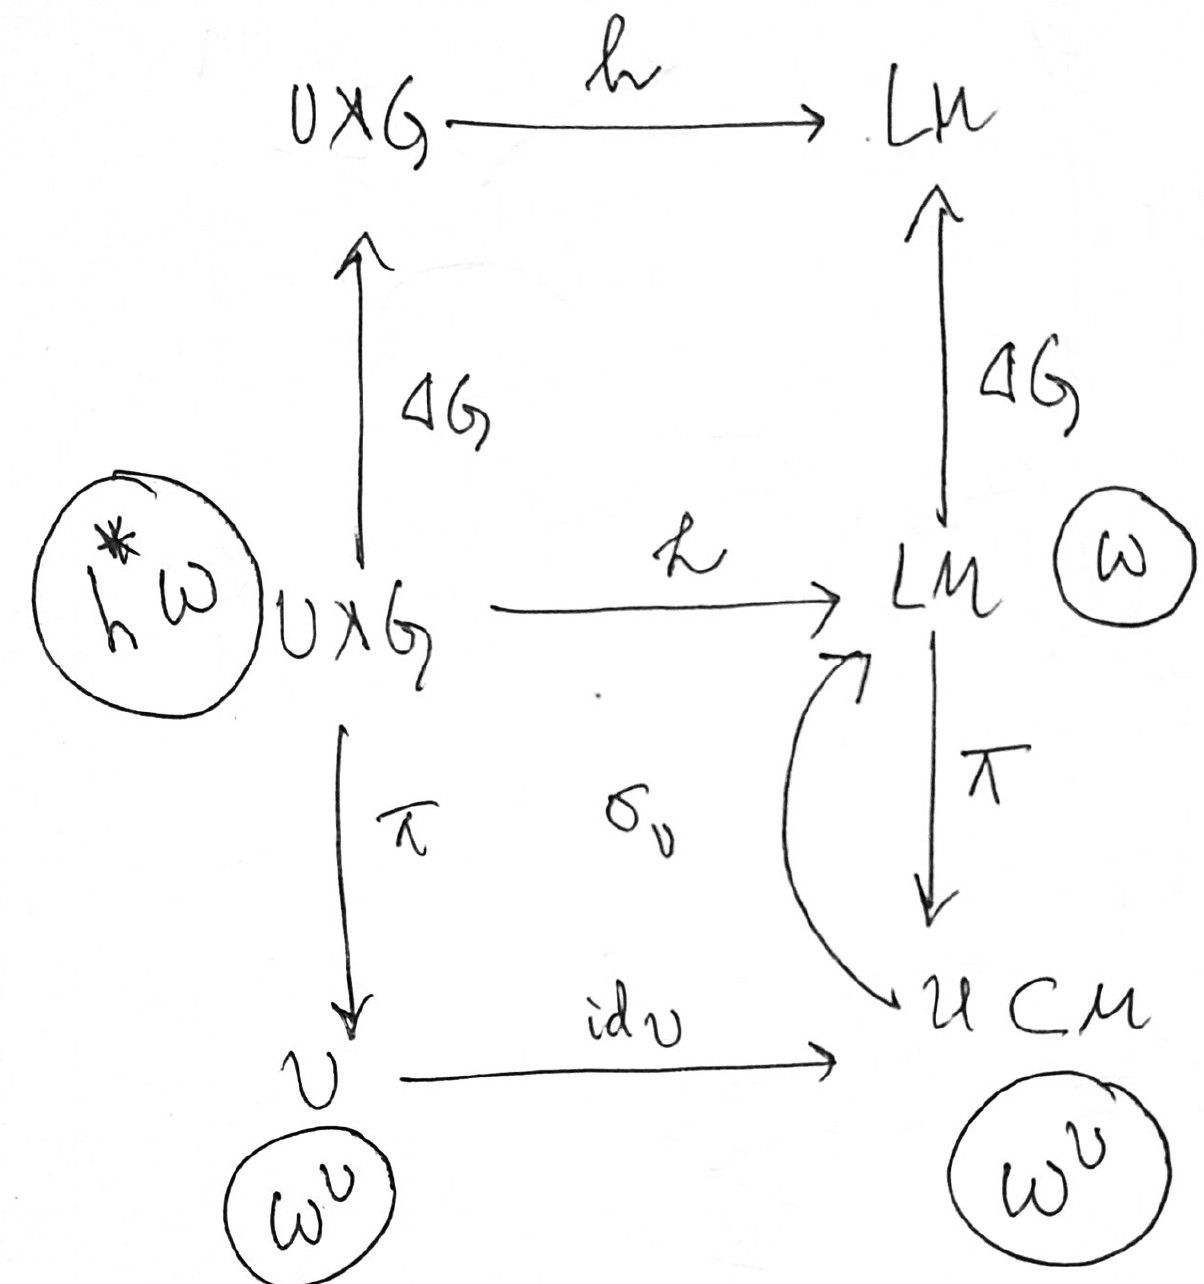
\includegraphics[scale = 0.1]{connection.jpg}
\caption{$\omega$ lives in total space, $\omega^{U}$ its chart-dependent projection over the manifold, loosing all its bundle-information (maurer-cartan form), and ${(h^{*}\omega)}$ which lives in a bundle section based on some local chart dependent trivialization, which provides us complete information so far about the bundle structure}
\end{center}
\end{figure}

\subsection{Horizonal Lift - Parallel Transport:} 

Suppose there is a curve over the base manifold $\gamma: t\in[0,1] \to M$. Now as discussed in the introduction of connection, in order to be able to compare two vectors in the total space, one must move from one tangent space to another, parallel to the curve at each instance, but can one ensure the parallelity in the total space, of a curve which is down to the base manifold, in order for than one needs to $Horizontally \ lift$ the curve from the base to the bundle space, and follow its pointwise tangent to move parallely. But the idea of Horizontal lift of a curve requires attention then. 

$\textbf{Definition:}$ Let $\gamma: t\in[0,1] \to M$ with $\gamma(0)=a ,\ \gamma(1)=b$ a curve in the base manifold, then the unique curve $\gamma^{\uparrow} : [0,1] \to P$ through a point $\gamma^{\uparrow}(0) = p \in \pi^{-1}(\{a \})$, which satisfies:

\begin{itemize}
\item $ \pi \circ \gamma^{\uparrow} = \gamma$

\item $ver(X_{\gamma^{\uparrow}, \gamma^{\uparrow}(\lambda)}) = 0  \ \ \forall \lambda \in [0,1]$

\item ${(\pi)}_{*}(X_{\gamma^{\uparrow}, \gamma^{\uparrow}(\lambda)}) = X_{\gamma, \gamma(\lambda)}$
\end{itemize}
Is called the Horizontal Lift of $\gamma$ through $p \in \pi^{-1}(\{a \})$. But how can one $explicitly \  evaluate \  the  \ horizontal \  lift$ of a curve for a given one. There are some short steps for that. 
Methods in sequential manner is discussed in the following. The outline sketch is as follows: first one needs to consider an arbitrary curve on the total space, such that its projection under $\pi$ projects down to the curve we want horizontally lift. There are infinite equivalence class of such curves possible \footnote{one can imagine it as following: draw a curve over a paper, and now arrange some sticks at several points of over the curve. Now, no matter how you put a line of thread tying up the sticks over the curve, it orthogonal projection, or just a shadow from perpendicularly shed torch will be the same curve.}. thus from each point from that arbitray curve, by moving suitably within the fibre by the right-action of the Lie Group, one obtains the exact horizontal lift. \footnote{just like moving the thread certainly at specific points one the sticks, one gets an unique horizontal lift, as both the curve now looks identical when fixed any point over the sticks, which are fibres here.}

$\textbf{i)}$ Consider an aribitrary curve $\delta: [0,1] \to P$ such that $\pi \circ \delta = \gamma \in M$ by action of a suitable curve $g: t \in [0,1] \to G$ such that 

\begin{align}{\label{arbitrarycurvetransport}}
\gamma^{\uparrow}(\lambda) = \delta(\lambda) \vartriangleright g(t)
\end{align}

\begin{figure}[h!]{\label{fig: hdhfjfdihfhdf}}
\begin{center}
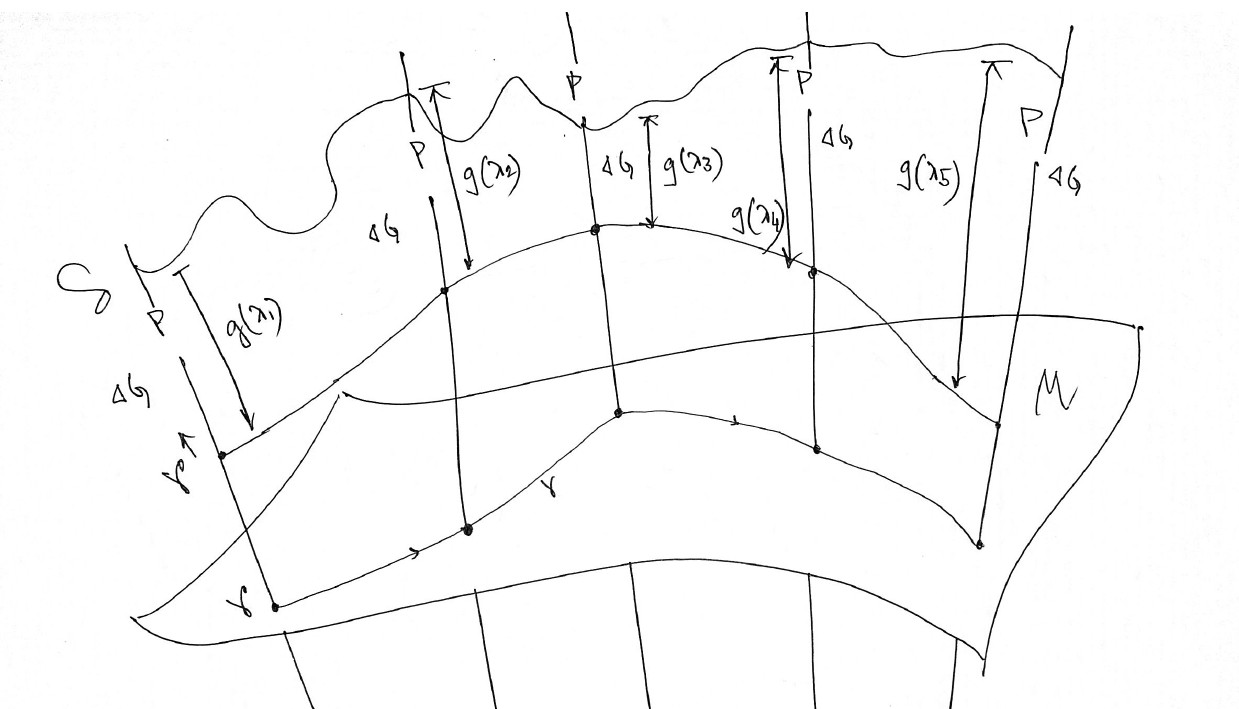
\includegraphics[scale = 0.15]{horizontallift.jpg} 
\hspace{0.3in}
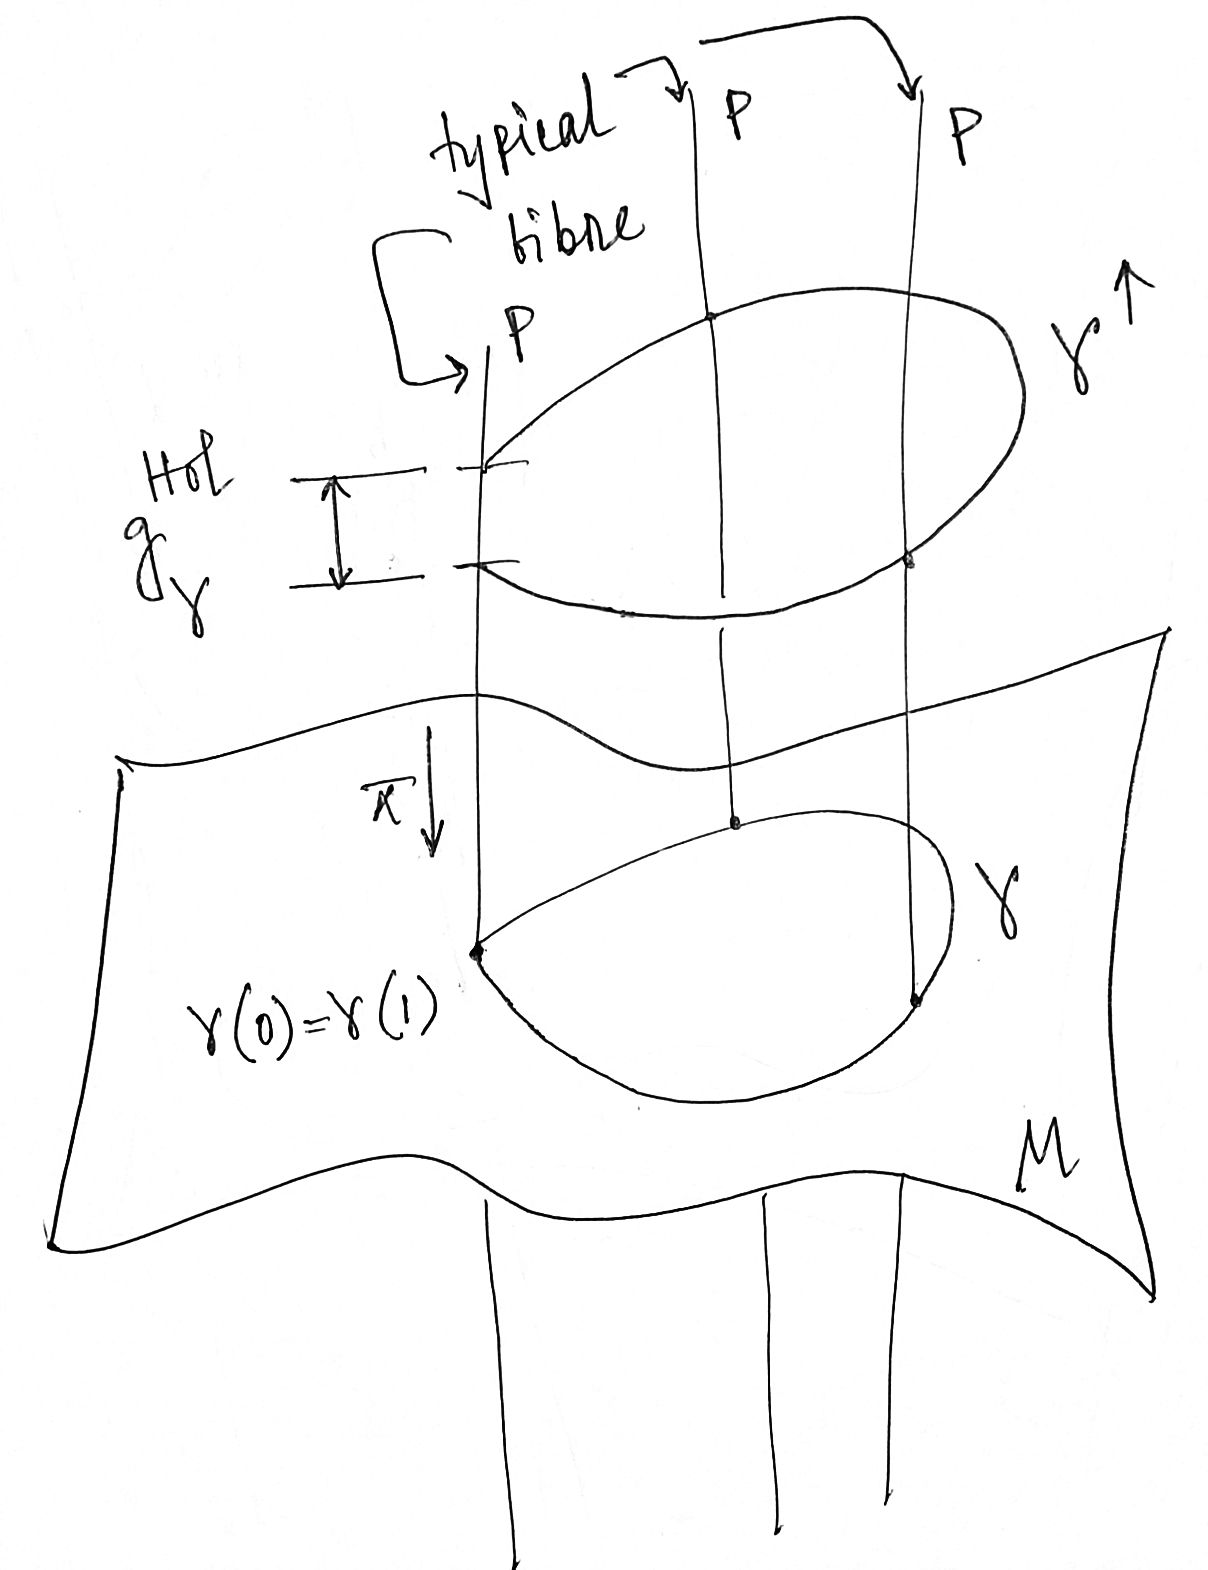
\includegraphics[scale = 0.1]{holonomy.jpg}
\caption{$\textbf{a)}$ $\gamma^{\uparrow}$ being the horizontal lift of $\gamma$ with the help of any arbitrary $\delta$ and corresponding group element variation ass $g(\lambda)$ 
$\textbf{b)}$  holonomy associated with closed curves} 
\end{center}
\end{figure}

$\textbf{ii)}$ the curve over the lie group requires to be the solution of a ODE with initial conditions as $g(0) = g_0 \in G$ for some element which is unique such that $\delta(0) \vartriangleright g_0 = p = \gamma^{\uparrow}(0)\in P $

Now from \ref{localyangmillsfield} and noting that $g(t)$s all belong the vertical subspaces, and $Horizontally \ lifted$ curve only has the Horizontal component and no vertical component, thus from \ref{jsafidsf}, 

\begin{align}
    & {(h^{*}\omega)}_{(m,g)}(({\pi}_{*}\delta), \gamma^{\uparrow}) = 0 \\
    & \implies {g(\lambda)}^{-1} {(\omega^{U}(X_{({\pi}_{*}\delta),}))}_{p} \ g(\lambda)+ {g(\lambda)}^{-1} \ \dot{g}(\lambda) = 0 \\
    & = {g(\lambda)}^{-1} \  {(\omega^{U}(X_{\gamma(\lambda)}))}_{p} \ g(\lambda)+ {g(\lambda)}^{-1} \ \dot{g}(\lambda)
\end{align}

With noting that $(X_{\delta(\lambda)}) =: ({\pi}_{*}\delta)$ which is the pushforward of the $\delta$ curve which lies on the total space, and also \footnote{the differential from \ref{coordinatedecomposition} the differential turns time derivative and one can consider $\underset{\delta t \to 0}{lim}$ of the expression}

Thus the ODE for characterizing the unique horizontal lift through a specific point over the fibre is:

\begin{align}
    {(\omega^{U}(X_{\delta(\lambda)}))}_{p} \ g(\lambda)+ \dot{g}(\lambda) = 0
\end{align}

Since we are considering local actions and manipulations of the one form, so choose a local section which will be pretty useful in dealing with $ {(\omega^{U}(X_{\delta(\lambda)}))}_{p}$. Consider a local section $\sigma : M \to P \ $, $ \pi \circ \sigma = id_M$ therefore the curve $\delta(\lambda)$ can as:

\begin{align}
    \sigma_{*}(X_{\gamma(\lambda)}) = X_{\delta(\lambda)}
\end{align}

Also from \ref{localconnectiononeform} and similar to \ref{coordinatedecomposition} we can decompose the one form as components and local one forms, since the local trivialization of the section allows one to do that: (for notational familiarity, with Connection Coefficients from General Relativity)

\begin{align}{\label{connectioncoeffeiahfpsfdsfdasgs}}
    \sigma^{*}(\omega) =  \omega^{U} = {\omega^{U}}_{\mu} \ dx^{\mu} = \Gamma_{\mu}dx^{\mu}
\end{align}
 Thus:

\begin{align}
    \omega^{U}(X_{\delta(\lambda)}) & =  {\Gamma_{\mu}} dx^{\mu} \ X^l \frac{\partial }{\partial x^l} \\
    &=  {\Gamma_{\mu}} \ X^l \ \delta^{\mu}_l = {\Gamma_{\mu}} X^{\mu}
\end{align}

Since $X$ is the vector field of the curve \footnote{the tangent to the curve at each point indeed corresponds to a vector field, consider the flow of water as an example, every flow-curve corresponds to a vector field} $\gamma$. Therefore componenwise $X^{\mu} = \dot{\gamma} = \frac{d \gamma}{d\lambda}$ where $\lambda$ is the parameterization of the curve and throughout this subsection, overhead dot represents derivative w.r.t. parameterization.

therefore the ODE simplifies to: 

\begin{align}{\label{veryeryimp}}
\dot{g}(\lambda) = - \Gamma_{\mu} \dot{\gamma}^{\mu} g(\lambda)
\end{align}

One cannot in general just take $g(\lambda)$ down to $dg(\lambda)$ and consider $d(ln(g(t)))$, since these are not ordinary function, but group elements which also are smooth functions, so the most general approach must be considered, for the sake of respecting its speciality. Therefore similar to what has been done at \ref{pathorderedintegral} it requires to be a path ordered integral since $\Gamma$s themselves are Lie-Algebra valued one form and componentwise sends vectors from local charts of the manifold to the Lie Algebra (which also is a vector space indeed) of the Lie Group which constitute each fibre of our whole construction, thus for general case for non-abelian Lie Groups one considers $path \ ordered \ integral$ as from the above expression, also :

\begin{align}
    g(t)& = g_0 - \int_{0}^{\lambda}  \Gamma_{\mu} \dot{\gamma}^{\mu} g(\lambda)d\lambda \\
    & =  g_0  \left[ 1 - \int_{0}^{t} d\lambda \Gamma_{\mu} \dot{\gamma}^{\mu} +  \int_{0}^{t} d\lambda \int^{\lambda}_{0} d\lambda_1 \dot{\gamma}^{\mu}(\lambda)\dot{\gamma}^{\mu}{\lambda} \Gamma_{\mu}(\lambda) \Gamma_{\mu}(\lambda_1)  - . . . \right] \\
    &= g_0 \left[  1 - \int_{0}^{t} d\lambda \Gamma_{\mu} \dot{\gamma}^{\mu} +  \frac{1}{2}\int_{0}^{t} d\lambda \int^{t}_{0} d\lambda_1 \dot{\gamma}^{\mu}(\lambda)\dot{\gamma}^{\mu}{\lambda} \Gamma_{\mu}(\lambda) \Gamma_{\mu}(\lambda_1)  - . . . \right] \\ 
    &=  \mathcal{P} \ exp \left[ - \int_{0}^{t} d\lambda \Gamma_{\mu} \dot{\gamma}^{\mu}\right] g_0= \mathcal{P} \ exp \left[ - \int_{0}^{t} \Gamma_{\mu} d\gamma^{\mu}\right] g_0
\end{align}


Where the $\mathcal{P}$ denotes a path ordered sign since in general $\Gamma_{\mu}(\lambda_i) \Gamma_{\mu}(\lambda_j) \neq \Gamma_{\mu}(\lambda_j) \Gamma_{\mu}(\lambda_i)$, i.e. they might not commute. \footnote{in case of our U(1) fibre bundle the path ordering will not at all be an issue since U(1) is abelian thus well commutative elementwise, here the most general expression has been presented} 

And thus from \ref{arbitrarycurvetransport} we finally obtain the most important result of this section, i.e., the $\textbf{horizontal lift}$ $\gamma^{\uparrow}$ is now given as, precisely from the figure \ref{hdhfjfdihfhdf}: with noting that $\delta(\lambda) = (\sigma \circ \gamma)(\lambda)$ as it is section induced:

\begin{align}
    \gamma^{\uparrow}(\lambda) = (\sigma \circ \gamma)(\lambda) \vartriangleleft \mathcal{P} \ exp \left[ - \int_{0}^{t} \Gamma_{\mu} d\gamma^{\mu}\right] g_0
\end{align}

Which precisely suffices the definition of Horizontal lift from the way it has been constructed. Now very importantly, I think it can be lot more simplified at this point, considering the arbitrary curve considered previously $\delta$ can also be chosen the curve one the base itself i.e. $\delta(\lambda) = \gamma(\lambda)$ since everything that lies on the base manifold, also is a part of the fibre-space and the section map can thus be constructed such that $\sigma \circ \gamma = \gamma$, then the above expression much more simplifies to:

\begin{align} {\label{horihorihorizontalliftkori}}
    \gamma^{\uparrow}(\lambda) = \gamma(\lambda) \vartriangleleft \mathcal{P} \ exp \left[ - \int_{0}^{t} \Gamma_{\mu} d\gamma^{\mu}\right] g_0
\end{align}
Isn't this a really beautiful expression. 

keeping in mind  that $g_0$ is such a group element that specifies the initial conditions i.e. $\gamma^{\uparrow}(0)  = \gamma \vartriangleright g_0$ which  also respects $\gamma(0) = \pi(\gamma^{\uparrow}(0) \vartriangleright g_0)$. One can find immediate relation with the $\textbf{Berry's Curvature}$ mentioned in the previous section. 

Now, after constructing the horizontal lift, parallel transport is nothing but, given a curve on the base manifold, going from a point to another over following the horizontal lift of the curve. Therefore:

$\textbf{Definition:}$ The parallel transport for a given curve is the map:

\begin{align}
    T_{\gamma}:& \pi^{-1}(\{ \gamma(0)\}) \to \pi^{-1}(\{ \gamma(1)\}) \\
    & \gamma^{\uparrow}(0) \mapsto \gamma^{\uparrow}(1)
\end{align}

It can also be given in terms of Covariant Derivative ($D$) as: (given a vector field $X$, in a simpler way):

\begin{align}{\label{covariantderivative}}
DX = dX + \omega^U(X) = dX + \Gamma_{\mu}X^{\mu}
\end{align}

and componentwise it turns out to be: 

\begin{align}
    D_jX^i = d_jX^i + {\Gamma_{\mu}}^i_jX^{\mu}
\end{align}

for the Lie Group being general Matrix Group, like $SO(3,1)$ for General Relativity and the Principal Fibre Bundle being the Frame Bundle mentioned here.

\subsection{Holonomy:}
It concerns us what happens when the curve is a loop over the base manifold, does its horizontal lift also make a loop it the total space! partly yes! but actually No. What actually happens, for a curve $\gamma:[0,1] \to M$ being a loop, i.e. $\gamma(0) = \gamma(1) = m \in M$ its horizontal lift $\gamma^{\uparrow}$ does indeed return to the same fibre it started from i.e. $\pi(\gamma^{\uparrow}(0)) = \pi(\gamma^{\uparrow}(0)) = \gamma(0) = \gamma(1) = m $ but it might change its position over the fibre, i.e. from \ref{horihorihorizontalliftkori} :

\begin{align}{\label{bahbahbahbah}}
    \gamma^{\uparrow}(1) = \gamma(1) \vartriangleright  \mathcal{P} \ exp \left[ - \oint \Gamma_{\mu} d\gamma^{\mu}\right] g_0 = \gamma^{\uparrow}(0) \vartriangleright  g_{\gamma}^{Hol}
\end{align}

as \footnote{since $\gamma(1) = \gamma(0)$ in the base manifold, and $\gamma^{\uparrow}(0) = \gamma(0) \vartriangleright g_0$} which immidiately says: from \ref{exponentialmap} $g_{\gamma}^{Hol} = \mathcal{P} \ exp \left[ - \oint \Gamma_{\mu} \gamma^{\mu}\right] g_0 \in G$ is the change in the fibre, i.e. not being able to close the loop in the fibre-space in general. 

This element $g_{\gamma}^{Hol}$ is called the $\textbf{Holonomy}$ associated with the curve $\gamma$ is as:

\begin{align}{\label{exactholonomy}}
    g^{Hol}_{\gamma} = \mathcal{P} \ exp \left[ - \oint \Gamma_{\mu} d\gamma^{\mu}\right] g_0
\end{align}

which one can strikingly find the relevence with the expression from Berry's Phase, with just the connection coeffecient being Electromagnetic Vector Potential \footnote{actuall it MUST be Electromagnetic Covector-potential}.


\subsection{Interpreting Geometric Phase as Holonomy:}
First proposed by B.Simons \cite{simon} the holonomic interpretation of the Geometric phase just some times after M.V.Berry's paper on geometric phases in adiabatic evolution. Although the interpretation consisted of adiabaticity, for cyclic evolution of some quantum system, thus clearly consisted of adiabatic approximation. It was $Aharanov \ Anandan$ who first showed the existance of geometric phase even for NO-adiabatic requirement, but just cyclic evolution of the quantum state in the $Projective \ Hilbert \ Space$ in  their famous paper $Phase \  change  \ during \  a  \ cyclic \  quantum  \ evolution$ \cite{aharanovanandan}. 

In that paper, the authors interpreted the evolution of a quantum system in the Hilbert Space, which projects down to a closed curve over Projective Hilbert Space $\mathcal{Ph}$, and the system is transported parallely with respect to the given evolution curve on $\mathcal{PH}$, and the holonomy thus generated turns out to be the Geometric Phase discussed earlier. Further on it will be demonstrated how this $\textbf{Aharanov-Anandan Phase}$ transforms into $Berry's \ Phase$ under adiabatic assumption. But for that the defintions and construction of the Principal Fibre Bundle of Aharanov-Anandan's 1987 work will be laid out. First the general approach will be considered and will then be specifically applied to Aharanov-Bohm Effect.

$\textbf{Definition:}$ Projective Hilbert Space is the equivalence class of state-vectors of Hilbert Space which are multiples are scalars. i.e.


\begin{align}
    \mathcal{PH} := \{ \ket{\psi} \sim \ket{\psi'} \in \mathcal{H}| \ket{\psi} = z \ .\  \ket{\psi'} \ \forall z \in \mathbb{C}\}
\end{align}

and the normalized state vectors over $\mathcal{PH}$ is given as:

\begin{align}
     \mathcal{PH}_{N} := \{  \ket{\psi} \in \mathcal{H}| \braket{\psi | \psi } = 1\} \simeq \{ \ket{\psi}\bra{\psi}, \ \ket{\psi} \in \mathcal{H} | \braket{\psi | \psi } = 1\}
\end{align}

One can just similarly interpret the normalized projective hilbert space as the space of pure-eigenprojectors as expressed above. 

One can readily see, from \ref{principalfibrebundledefinition} The hilbert space here is the $total \ Space$, the $U(1)$ Lie Group as each fibre,  $\mathcal{PH}_N$ since every element of it are related to corresponding rays in $\mathcal{H}$, Since every  elements in $\mathcal{H}$ are related to an arbitrary phase factor $e^{i\alpha} \in U(1)$ which projects down to $\mathcal{PH}_N$ at the same spot.

Therefore Construct the Principal Fibre Bundle and just call it $Hilbert \ Bundle$ since it is indeed so:

\begin{align}
(\mathcal{H}, \mathcal{PH}_N, \pi, U(1))
\end{align}
Where from the definition of principal Fibre Bundle \footnote{
note Hilbert space being treated as $\mathbb{R}^n$, $\mathcal{PH} \equiv {\mathbb{C}P}^{n-1}$ and infinite dimension case both are infinite dimensional and indeed for either the cases they are manifolds themselves} as \ref{principalfibrebundledefinition} There is a surjective projection map $\pi: \mathcal{H} \to \mathcal{PH}_N$\footnote{this projection map cannot be injective, then the total space will be isomorphic to the base space, and fibres will be none but just a point} is defined as: \footnote{one thing as well, the U(1) group is an abelian group thus the left and right actions of the group elements can be treated equivalently}

\begin{align}
    \pi(e^{i\alpha} \ket{\psi}) := \ket{\psi} \in \mathcal{PH}_N \ \ \ \forall \alpha \in \mathbb{R}
\end{align}

From this point on $\ket{\bar{\psi}}$ would be denoted explicitly for an element of $\mathcal{PH}$ which is clearly in $\mathcal{H}$ for $\alpha = 0$ or simply no phase at all and regular state vector $\ket{\psi}$ lives in $\mathcal{H}$.

Now consider a Hamiltonian $H(t)(\hat{p}, \hat{r}) \equiv H(\frac{\hbar}{i}\nabla, r(t))$ written in position-space representation. And consider a system, evolving as a solution of Schrodinger equation maintaining this hamiltonian: [for the moment no electromagnetic field is being introduces, just standard kinetic and potential stuff]

\begin{align}
    i\hbar\frac{d}{dt} \ket{\psi(t)} = H(t) \ket{\psi(t)}
\end{align}
clearly from \ref{axiom1} the evolution of state, an additional phase factor would accompany its dynamical evolution, namely just the dynamical phase say $\eta_d$. For a closed evolution of $\ket{\psi(t)}$ can be given as:  [in other words $\ket{\psi(t)}$ lives in $\mathcal{PH}$ and for cyclic evolution does indeed complete a closed curve, BUT upto a phase and $t \in [0-\tau]$ is considered the time range for cyclicity]

\begin{align}{\label{pihere}}
    & \pi(\ket{\psi(\tau)}) = \pi(\ket{\psi(0)}) = a \in \mathcal{PH} \\ 
    & \ket{\psi(\tau)} = \ket{\psi(0)} \  e^{i \eta_d}
\end{align}

Now construct:

\begin{align}{\label{newhorihori}}
    \ket{\bar{\psi}(t)}= \ket{\psi(\tau)} \ e^{-if(t)}
\end{align}

such that: $f(\tau) - f(0) = \eta_d$ and then one readily sees $\ket{\bar{\psi}(\tau)} = \ket{\bar{\psi}(0)}$ and this has been constructed such that $\ket{\bar{\psi}(t)}$ indeed lives down the $\mathcal{PH}$ and does form a closed loop there. It is exactly like \ref{arbitrarycurvetransport} where the group elements are as: $g(t) \in G \to e^{-if(t)} \in U(1)$ and this is where the whole thing come together regarding developments of previous sections, rather as argued before the arbitrar curve $\delta$ could be the curve over the base manifold which here is the $\mathcal{PH}$ where $\delta$ can be considered to the curve $\ket{\bar{\psi}(\tau)}$ itself, thus from the relation \ref{arbitrarycurvetransport}

\begin{align}
    \delta  = \ket{\bar{\psi}(\tau)}  \ \ \ \ \gamma^{\uparrow} = \ket{\psi(\tau)} \ \ \ \ g(t) = e^{-if(t)} \ \ \ \ G = U(1)
\end{align}
This completes the construction. And which clearly means, at each instance of the time, for $\ket{\bar{\psi}(t)}$ to maintain Schrodinger Equation, it must go up or down the fibre at amount  $e^{-if(t)}$, and the solution itself is the curve over the total space $\mathcal{H}$. Thus putting \ref{newhorihori} in Schrodinger equation, we get an ODE of the the Lie Algebra Elements $f(t)$ \footnote{Lie Algebra of U(1) is $\mathbb{R}$ as one can see from $\mathfrak{X}(G) \simeq T_eG$ the tangent space of a Unit Circle $S^1 \equiv U(1)$ is nothing but the real line}. takes the form after taking inner product of the expression with $\bra{\bar{\psi}(t)}$: \footnote{Here the Schrodinger Equation determines the evolution of the group elements f(t)} as \cite{aharanovanandan}

\begin{align}
    & -\frac{df}{dt} = \frac{1}{\hbar} \braket{\psi(t)|H|\psi(t)} - i \braket{\bar{\psi}(t)|\frac{d}{dt}|\bar{\psi}(t)}\\ 
    & \implies f(t) = \frac{i}{\hbar} \int_0^{t} \braket{\psi(t')|H|\psi(t')} dt' + i  \int_0^{t}\braket{\bar{\psi}(t')|\frac{d}{dt'}|\bar{\psi}(t')}dt' \\ 
    &= \frac{i}{\hbar} \int_0^{t} \braket{\psi(t')|H|\psi(t')} dt' + i  \int_{x_0}^{x_t}\braket{\bar{\psi}(t')|\nabla_{\mu}|\bar{\psi}(t')}dx^{\mu} 
\end{align}

Where the Geometric phase now peeks in. As constructed, for such this cyclic evolution where $f(\tau)= f(0) + \eta_d(\tau)$, thus for the curve over on the total space, being the horizontal lift of the curve on $\mathcal{PH}$ as considered the solution of Schrodinger equation, transforms as, for $\textbf{cyclic evolution}$, noting that for closed evolution $x(0) = x(\tau)$ which are coordinate patches over $\mathcal{PH}$

\begin{align}
    \ket{\psi(\tau)} &= e^{i \eta_d(\tau)} \ket{\psi(0)}\\
    &= e^{i(f(\tau)) - f(0))} \ket{\psi(0)} \\ 
    &= exp  \left[   \frac{i}{\hbar} \int_0^{\tau} \braket{\psi(t')|H|\psi(t')} dt' + i  \oint \braket{\bar{\psi}(t')|\nabla_{\mu}|\bar{\psi}(t')}dx^{\mu}  \right]\ket{\psi(0)} 
\end{align}

Clearly it seems now, for the projection map $\pi: \mathcal{H} \to \mathcal{PH}$ from \ref{pihere} both $\ket{\psi(\tau)}$  and $\ket{\psi(0)}$ down to the same point on $\mathcal{PH}$ but when one compares it with \ref{bahbahbahbah} one immidiately finds the phase factor to have been accumulated with the parallel transport over the curve on $\mathcal{PH}$ of which the first one is familiarly as dynamical part, and another part. 

Now defining:

\begin{align}
    \beta =   \oint i \braket{\bar{\psi}(t')|\nabla_{\mu}|\bar{\psi}(t')}dx^{\mu} 
\end{align}

One can see for arbitrary phase transformations of $\bar{\psi}(t')$ the contour integral is invariant, just as was discussed in \ref{gaugeinvariance11}. Therefore the additional phase part $\beta$ $\textbf{for cyclic evolution}$ cannot be discarded away for its gauge invariance character, BUT for regular non-cyclic evolution one can consider a phase transformation and remove it away, just that's why this fundamental aspect of phase in quantum theory, especially for cyclic evolution, took physicists many years to consider thoroughly. 

In case of Aharanov-Bohm effect, there are two possible ways to consider the situation, and relate to the developements made so far, but things become much easier when written down the Schrodinger equation in terms of Covariant Derivative as \ref{covariantderivative}:

\begin{align}{\label{electromagneticschrodingereequatinon}}
\begin{split}
     i\hbar \frac{d}{dt} \psi ={}& {(\frac{\hbar}{i} \nabla)}^2 \psi
\end{split}\\
\begin{split}
   	\downarrow
\end{split}\\
\begin{split}
    i\hbar (\frac{d}{dt} + \frac{q}{c} A_0) \psi' ={}& -{\hbar}^2{( \nabla - \frac{qi}{hc} A) }^2 \psi'
\end{split}
\end{align}

With $A_0 = cV$ the scalar potential, and $A$ being the (Co-)vector potentaial. Therefore transforming our derivarives as:

\begin{align}{\label{againemconnection}}
    \frac{d}{dt} \mapsto D_0 := \frac{d}{dt} + \frac{q}{c} A_0 \ \ \ \ \ \nabla \mapsto D_{\alpha}:=\nabla - \frac{iq}{hc} A 
\end{align}

Thus the covariant-Schrodinger equation takes the form:

\begin{align}
    i\hbar D_0 \psi = {(\frac{\hbar}{i} D_{\alpha})}^{2}\psi
\end{align}

Where the Electromagnetic Potentials played the role of Local Connection Coefficients as from \ref{connectinemememe} and \ref{covariantderivative}. Therefore from \ref{bahbahbahbah} ignoring the dynamical phase factor: one obtains for the Closed loop evolution, that:


\begin{align}
    \ket{\psi_f} = exp \left[ \frac{iq}{hc} \oint A_{\mu}dx^{\mu} \right] \ket{\psi_i}
\end{align}

Where $i, j$ represents initial and final states, which one finds exactly same to be as \ref{abphase} just written componentwise, but obtained from very different argument, which indeed is the $\textbf{Aharanov-Bohm Phase}$.


    


\section{conclusion:}

It's just another example of 'unreasonable effectiveness of mathematics in natural science' as Mr. Wigner has mentioned.


\documentclass[8pt, a4paper]{article}
	\usepackage[left=2.5cm, right=2.5cm, top=2.5cm, bottom=1.5cm]{geometry}

    \title{\textbf{Geometric Phase in Quantum Theory: 
    \\ It's relevence from Schrödinger to Schwarzschild}}
    
    
    \author{}
    \date{I don't know when.07.2021}
    

\usepackage{amsmath}
\usepackage{amsthm}
\usepackage{amsfonts}
\usepackage{amssymb}
\usepackage{hyperref}
\usepackage{chngcntr}
\usepackage{braket}
\usepackage{esint}
\usepackage{graphicx}




\begin{document}
\begin{thebibliography}{}

\bibitem[1]{schuller} \href{https://mathswithphysics.blogspot.com/2016/07/frederic-schullers-lectures-on-quantum.html}{Lectures on Quantum Theory by Frederic P. Schuller Friedrich-Alexander-Universität Erlangen-Nürnberg (FAU)}
 
 \bibitem[2]{adiabaticberry} \href{https://ethz.ch/content/dam/ethz/special-interest/phys/theoretical-physics/itp-dam/documents/gaberdiel/proseminar_fs2018/05_Stengele.pdf}{Sebastian Stengele - Berry's Phase - Proseminar - Algebra, Topology, and Group Theory in Physics 2018}
 
 \bibitem[3]{berrypaper}\href{https://www.jstor.org/stable/2397741}{Quantal Phase Factors Accompanying Adiabatic Changes: 
M. V. Berry Proceedings of the Royal Society of London. Series A, Mathematical and Physical Sciences
Vol. 392, No. 1802 (Mar. 8, 1984), pp. 45-57 (13 pages)
Published By: Royal Society}

 \bibitem[4]{ab}\href{}{Significance of Electromagnetic Potentials in the Quantum Theory Y. Aharonov and D. Bohm}
 
 
 \bibitem[5]{geop}\href{}{The Geometric Phase in Quantum Systems  Bohm, A., Mostafazadeh, A., Koizumi, H., Niu, Q., Zwanziger, J}
  
  \bibitem[6]{pathAharonov}\href{}{Feynman path-integral approach to the Aharonov-Bohm effect
Christopher C. Gerry and Vijay A. Singh}

	\bibitem[7]{goodone} \href{https://physik.uni-graz.at/~uxh/diploma/orasch14.pdf}{The Aharonov-Bohm-Effect: Oliver Orasch: Karl-Franzens-Universität Graz}
	
	\bibitem[8]{simon} \href{}{Holonomy, the Quantum Adiabatic Theorem, and Berry's Phase: B. Simon
Phys. Rev. Lett. 51, 2167 – Published 12 December 1983}

\bibitem[9]{geomanatomy} \href{https://www.youtube.com/playlist?list=PLPH7f_7ZlzxTi6kS4vCmv4ZKm9u8g5yic}{lectures on Geometrical Anatomy of Theoretical Physics: Frederic Schuller }

\bibitem[10]{doeslie} \href{https://math.uchicago.edu/~may/REU2016/REUPapers/Mandel.pdf}{What does the lie algebra know about the lie group: Holy Mandel}
  
  \bibitem[11]{aharanovanandan}\href{}{Phase change during a cyclic quantum evolution
Y. Aharonov and J. Anandan
Phys. Rev. Lett. 58, 1593}
  
 
\end{thebibliography}

\end{document}\
\end{document}